%! Author = crist
%! Date = 25/10/2026

\spacing{1.3}
%----------------------------------------------------------------------------------------
%	UNIDAD 6: LAS REACCIONES QUÍMICAS (4.º ESO)
%   Figuras: images/UD6/*.pdf (fuente HTML en images/UD6/html, SVG en images/UD6/svg)
%----------------------------------------------------------------------------------------

% Mapa conceptual del tema (fuente en images/mapas_conceptuales/html/temas.js)
\begin{figure}[H]
    \centering
    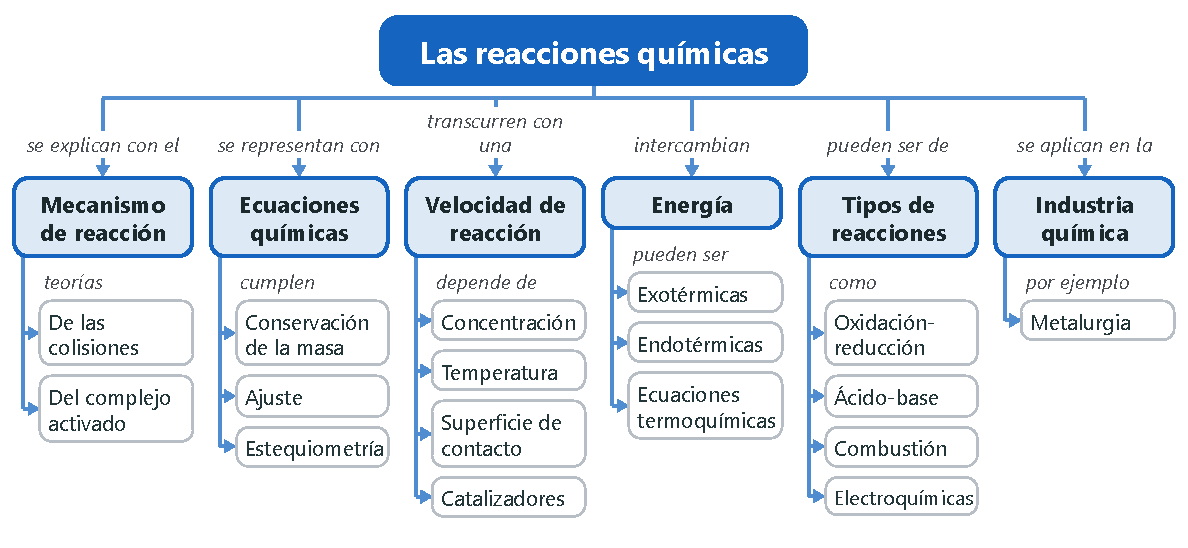
\includegraphics[width=\textwidth]{images/mapas_conceptuales/mapa_UD6}
\end{figure}

%========================================================================================
%\section*{Para empezar: el dióxido de carbono y el efecto invernadero}
%\addcontentsline{toc}{section}{Para empezar: el dióxido de carbono y el efecto invernadero}
%========================================================================================
%
%Antes de la Revolución Industrial, el aire contenía unas 280 partes por millón (ppm) de dióxido de carbono. El \ch{CO2} retiene cerca de la superficie parte del calor que la Tierra emitiría al espacio, y gracias a ese «termostato» la temperatura media del planeta se mantuvo en torno a \qty{14}{\celsius}: con ese clima construimos nuestras ciudades y aprendimos a cultivar.
%
%Cuando empezamos a quemar carbón, petróleo y gas para obtener energía, la cantidad de \ch{CO2} empezó a subir: en 2007 ya era de 380~ppm y en 2022 alcanzó las 420~ppm, el valor más alto desde que hay registros. El \ch{CO2} es un gas \textbf{persistente}: permanece mucho tiempo en la atmósfera y lo que se emite se va acumulando. El calentamiento resultante está fundiendo los hielos, cambiando las estaciones y el régimen de lluvias, y haciendo subir el nivel del mar.
%
%La principal reacción responsable es la \textbf{combustión}: \ch{C + O2 -> CO2}. Reducir sus emisiones está relacionado con los \textbf{ODS 7} (\emph{Energía asequible y no contaminante}), \textbf{11} (\emph{Ciudades y comunidades sostenibles}), \textbf{12} (\emph{Producción y consumo responsables}) y \textbf{13} (\emph{Acción por el clima}). Pero, además de las decisiones de los gobiernos, hará falta la acción de cada persona.
%
%\begin{exercise}
%    ¿Cuánto \ch{CO2} había en la atmósfera antes de la Revolución Industrial? ¿Por qué ha aumentado desde entonces? ¿Qué reacción química es la principal responsable?
%    \begin{solu}
%        Unas \textcolor{red}{280~ppm}. Ha aumentado por la \textcolor{red}{quema de combustibles fósiles} (carbón, petróleo y gas) en la industria, el transporte y la producción de energía. La reacción responsable es la combustión: \ch{C + O2 -> CO2}.
%    \end{solu}
%\end{exercise}
%
%\begin{exercise}
%    ¿Qué concentración de \ch{CO2} se midió en 2007 y en 2022? ¿Qué consecuencias del calentamiento se observaban ya en 2007? ¿Es fácil eliminar el \ch{CO2} acumulado?
%    \begin{solu}
%        \textcolor{red}{380~ppm} en 2007 y \textcolor{red}{420~ppm} en 2022: la situación no ha mejorado. Ya en 2007 se observaban la fusión de los hielos, cambios en las estaciones y en las lluvias y la subida del nivel del mar. No es fácil eliminarlo: es un gas \textcolor{red}{persistente}.
%    \end{solu}
%\end{exercise}
%
%\begin{exercise}
%    ¿Cómo pueden ayudar los ODS 7, 11, 12 y 13 a reducir los gases de efecto invernadero? ¿Qué puedes hacer tú?
%    \begin{solu}
%        Promueven energías limpias, ciudades sostenibles, un consumo responsable y medidas contra el cambio climático, todo lo cual reduce las emisiones. Respuesta libre para la acción individual: usar transporte público o bicicleta, ahorrar energía en casa, consumir productos locales, reciclar\ldots
%    \end{solu}
%\end{exercise}

%========================================================================================
\section{¿Cómo se produce una reacción? El mecanismo de reacción}
%========================================================================================

Si calentamos en una cápsula de porcelana una mezcla de aluminio y yodo, el conjunto arde con grandes llamas y al final queda un polvo blanco: una sustancia nueva, el triyoduro de aluminio:
\[ \ch{2 Al (s) + 3 I2 (s) -> 2 AlI3 (s)} \]
Para que ocurra, se han \textbf{roto} los enlaces metálicos del aluminio y los enlaces covalentes del yodo, y se han \textbf{formado} enlaces nuevos entre el aluminio y el yodo.

\begin{definition}[Reacción química y mecanismo de reacción]
    En una \textbf{reacción química} se rompen enlaces de las sustancias iniciales, los \textbf{reactivos}, y sus átomos se reorganizan formando enlaces nuevos para dar sustancias distintas, los \textbf{productos}. El conjunto de procesos elementales por los que transcurre se llama \textbf{mecanismo de reacción}.
\end{definition}

Dos teorías explican el mecanismo de las reacciones: la teoría de las colisiones y la del complejo activado.

\subsection{La teoría de las colisiones}

Según el modelo cinético de la materia, las partículas están en continuo movimiento. Para que reaccionen, las partículas de los reactivos (átomos, moléculas o iones) tienen que \textbf{chocar}. Pero no todos los choques sirven: un \textbf{choque es eficaz} solo si las partículas chocan
\begin{itemize}
    \item con \textbf{energía suficiente}: si no, se limitan a rebotar;
    \item con la \textbf{orientación adecuada}: aunque choquen con mucha energía, si no se orientan bien no pueden romperse los enlaces para formar los nuevos.
\end{itemize}

\begin{figure}[H]
    \centering
    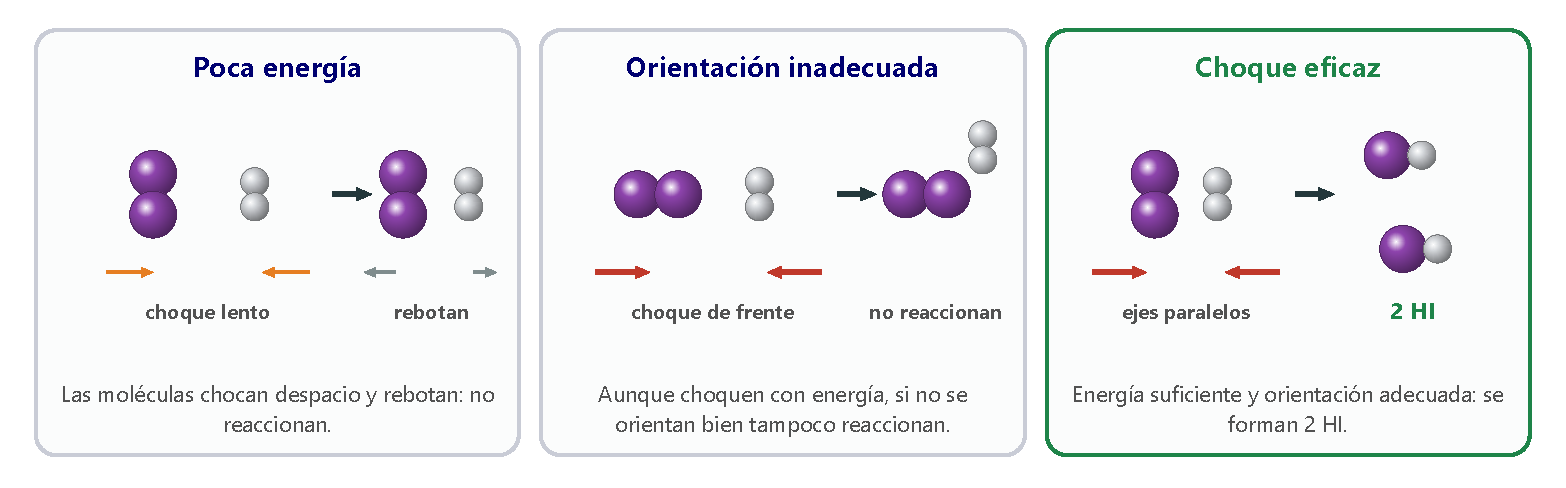
\includegraphics[width=\textwidth]{images/UD6/colisiones}
    \caption{Choques entre moléculas de \ch{I2} (moradas) y de \ch{H2} (grises). Solo el último es eficaz.}
    \label{fig:colisiones}
\end{figure}

\subsection{La teoría del complejo activado}

Cuando las partículas chocan con energía y orientación adecuadas, sus átomos pasan, durante un instante, por una agrupación inestable de alta energía: el \textbf{complejo activado}. En él, los enlaces de los reactivos se han debilitado y los de los productos han empezado a formarse. Desde ahí puede dar los productos o volver a dar los reactivos.

\begin{definition}[Energía de activación, \(E_a\)]
    Es la energía mínima que necesitan las partículas que chocan con la orientación adecuada para formar el complejo activado y que la reacción tenga lugar. En el diagrama de energía es la «barrera» entre los reactivos y el complejo activado.
\end{definition}

\begin{figure}[H]
    \centering
    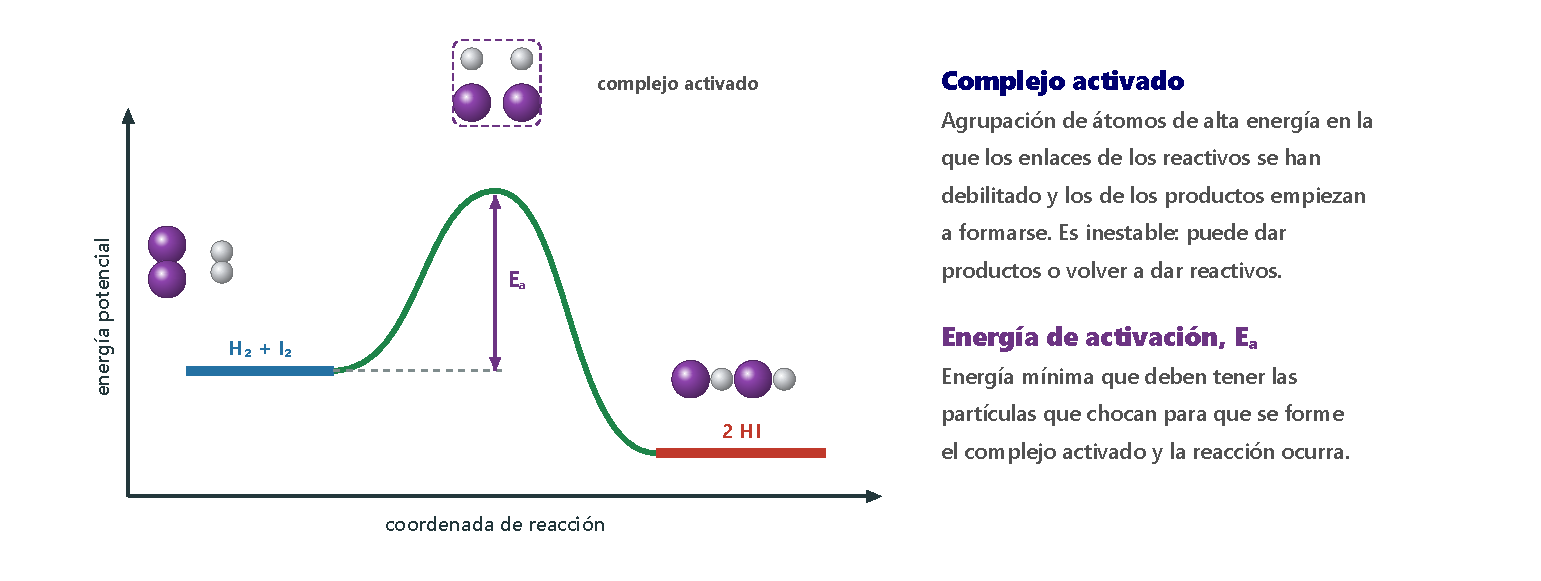
\includegraphics[width=\textwidth]{images/UD6/complejo_activado}
    \caption{Diagrama de energía de la reacción \ch{H2 + I2 -> 2 HI}.}
    \label{fig:complejo_activado}
\end{figure}

\begin{exercise}
    En la reacción \ch{NO + NO3 -> 2 NO2} la molécula de \ch{NO} tiene que unirse por su átomo de nitrógeno a uno de los oxígenos del \ch{NO3}. Explica cuál de estos choques podría dar lugar a la reacción:
    \begin{enumerate}[label=\alph*)]
        \item El \ch{NO} choca por su oxígeno con el nitrógeno del \ch{NO3}.
        \item El \ch{NO} choca por su nitrógeno con un oxígeno del \ch{NO3}.
        \item El \ch{NO} choca de lado, sin que ningún átomo quede enfrentado a un oxígeno del \ch{NO3}.
    \end{enumerate}
    \begin{solu}
        Solo el choque \textcolor{red}{b)}: es el único con la orientación adecuada, porque el nitrógeno del \ch{NO} queda enfrentado a un oxígeno del \ch{NO3} y puede formarse el enlace \ch{N-O}. (Además, tiene que producirse con energía suficiente.)
    \end{solu}
\end{exercise}

\begin{exercise}
    Relaciona cada concepto con su definición.

    \textbf{Conceptos:} a) Teoría de las colisiones. b) Teoría del estado de transición. c) Complejo activado. d) Energía de activación.

    \textbf{Definiciones:} A. Energía mínima necesaria para que reaccionen dos partículas que chocan con la orientación adecuada. B. Para que haya reacción, las partículas deben chocar con energía suficiente y orientación adecuada. C. Los átomos pasan por una distribución de enlaces menos estable que la de los reactivos y los productos. D. Agrupación de alta energía en la que los enlaces de los reactivos se han debilitado y los de los productos han empezado a formarse.
    \begin{solu}
        \textcolor{red}{a--B; b--C; c--D; d--A.}
    \end{solu}
\end{exercise}

\begin{exercise}
    Queremos subir una piedra desde un valle (A) hasta el otro lado de una colina, a un valle más bajo (B), pasando por la cima (C). ¿En qué se parece este trayecto al diagrama de energía de una reacción química?
    \begin{solu}
        La piedra en A son los \textcolor{red}{reactivos}; la cima C, el \textcolor{red}{complejo activado}; el valle B, los \textcolor{red}{productos}. Aunque B está más bajo que A, para llegar hay que «subir» primero la colina: esa subida es la \textcolor{red}{energía de activación}.
    \end{solu}
\end{exercise}

\begin{exercise}
    Indica qué enlaces se rompen y cuáles se forman en estas reacciones, y de qué tipo es cada enlace:
    \begin{enumerate}[label=\alph*)]
        \item \ch{H2 (g) + Br2 (g) -> 2 HBr (g)}
        \item \ch{2 H2 (g) + O2 (g) -> 2 H2O (g)}
        \item \ch{C (grafito) + O2 (g) -> CO2 (g)}
        \item \ch{Zn (s) + 2 HCl (aq) -> ZnCl2 (aq) + H2 (g)}
    \end{enumerate}
    \begin{solu}
        a) Se rompen \ch{H-H} y \ch{Br-Br}; se forman \ch{H-Br}. Todos \textcolor{red}{covalentes}.
        b) Se rompen \ch{H-H} y \ch{O=O}; se forman \ch{O-H}. Todos \textcolor{red}{covalentes}.
        c) Se rompen los enlaces \ch{C-C} del cristal de grafito (\textcolor{red}{covalente reticular}) y el \ch{O=O} (covalente); se forman \ch{C=O} (covalentes).
        d) Se rompen los enlaces del zinc (\textcolor{red}{metálico}) y los \ch{H-Cl} (covalentes); se forman la unión entre los iones \ch{Zn^{2+}} y \ch{Cl-} (\textcolor{red}{iónica}) y el \ch{H-H} (covalente).
    \end{solu}
\end{exercise}

\begin{exercise}
    Indica si son verdaderas o falsas y corrige las falsas:
    \begin{enumerate}[label=\alph*)]
        \item Para que haya reacción basta con que las partículas de los reactivos tengan energía suficiente.
        \item El complejo activado se forma cuando los reactivos chocan con energía y orientación adecuadas, y tiene más energía que los reactivos y los productos.
        \item La energía de activación es la energía mínima que necesitan las partículas que chocan con la orientación adecuada para reaccionar.
        \item Los reactivos siempre tienen menos energía que los productos.
    \end{enumerate}
    \begin{solu}
        a) \textcolor{red}{Falsa}: además deben chocar con la orientación adecuada. b) \textcolor{red}{Verdadera}. c) \textcolor{red}{Verdadera}. d) \textcolor{red}{Falsa}: eso solo ocurre en las reacciones endotérmicas; en las exotérmicas los productos tienen menos energía.
    \end{solu}
\end{exercise}

\begin{exercise}
    En la reacción \ch{NO3 (g) + CO (g) -> NO2 (g) + CO2 (g)} se observan tres choques: A) las moléculas se orientan bien pero chocan muy despacio; B) chocan con mucha energía pero el \ch{CO} golpea al nitrógeno; C) chocan con energía y el carbono del \ch{CO} se enfrenta a un oxígeno del \ch{NO3}. ¿Cuál es eficaz? ¿Por qué no lo son los otros?
    \begin{solu}
        Solo es eficaz el \textcolor{red}{C}: tiene energía suficiente y orientación adecuada. En A falta \textcolor{red}{energía} y en B falla la \textcolor{red}{orientación}.
    \end{solu}
\end{exercise}

%========================================================================================
\section{¿Qué sucede con la masa en una reacción química?}
%========================================================================================

En 1774, el químico francés Antoine-Laurent \textbf{Lavoisier} calentó estaño en un recipiente cerrado y comprobó que la masa total no cambiaba: el estaño se combinaba con el oxígeno del aire del recipiente para formar óxido de estaño, y lo que ganaba el metal era exactamente lo que perdía el aire.

\begin{definition}[Ley de conservación de la masa o ley de Lavoisier]
    En una reacción química la masa total del sistema permanece constante: la masa de los reactivos que reaccionan es igual a la masa de los productos que se forman.
\end{definition}

La teoría de las colisiones lo explica: en una reacción \textbf{los átomos no aparecen ni desaparecen}, solo se reorganizan; por tanto, la masa total se conserva (figura~\ref{fig:conservacion_masa}).

\begin{figure}[H]
    \centering
    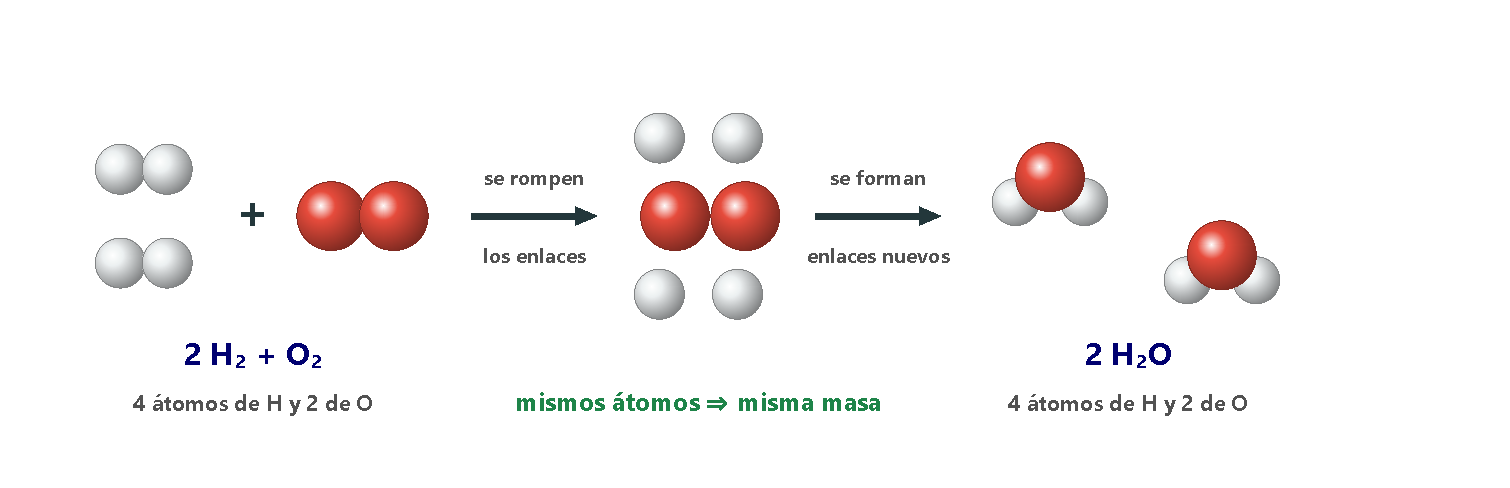
\includegraphics[width=\textwidth]{images/UD6/conservacion_masa}
    \caption{En la reacción \ch{2 H2 + O2 -> 2 H2O} los átomos se reorganizan, pero no cambia su número.}
    \label{fig:conservacion_masa}
\end{figure}

\begin{remark}
    \textbf{Otras dos leyes de las reacciones.} \emph{Ley de las proporciones definidas (Proust):} cuando dos elementos se combinan para formar un compuesto, lo hacen siempre en la misma proporción de masa. \emph{Ley de los volúmenes de combinación (Gay-Lussac):} los volúmenes de los gases que reaccionan y los de los gases que se forman, medidos en las mismas condiciones, están en una relación de números enteros sencillos.
\end{remark}

\begin{exercise}
    Para comprobar la ley de conservación de la masa en la maduración de la fruta, pesamos una manzana en un plato, la dejamos varios días y la volvemos a pesar.
    \begin{enumerate}[label=\alph*)]
        \item ¿Coincidirán la masa inicial y la final?
        \item ¿Qué cambiarías en el experimento?
    \end{enumerate}
    \begin{solu}
        a) \textcolor{red}{No}: la manzana pierde agua y gases (como \ch{CO2}) que escapan al aire, así que la masa final es menor. b) Habría que hacerlo en un \textcolor{red}{recipiente cerrado} para que no se pierdan los productos gaseosos (y controlar la temperatura y la humedad). Entonces la masa total sí se conservaría.
    \end{solu}
\end{exercise}

\begin{exercise}
    Al calentar \qty{23.2}{\gram} de óxido de plata en un recipiente abierto quedan \qty{21.6}{\gram} de plata.
    \begin{enumerate}[label=\alph*)]
        \item ¿Qué masa de oxígeno se ha desprendido?
        \item ¿Qué habría pasado en un recipiente hermético?
    \end{enumerate}
    \begin{solu}
        a) \(m_\text{oxígeno} = \num{23.2} - \num{21.6} = \textcolor{red}{\qty{1.6}{\gram}}\). b) La masa total del recipiente \textcolor{red}{no habría cambiado}, porque el oxígeno habría quedado dentro.
    \end{solu}
\end{exercise}

\begin{exercise}
    ¿Qué masa de carbono reacciona con \qty{16}{\gram} de oxígeno si se forman \qty{22}{\gram} de dióxido de carbono?
    \begin{solu}
        Por la ley de Lavoisier: \(m_\text{C} = 22 - 16 = \textcolor{red}{\qty{6}{\gram}}\).
    \end{solu}
\end{exercise}

%========================================================================================
\section{¿Cómo se escribe una ecuación química?}
%========================================================================================

Una \textbf{ecuación química} representa una reacción. A la izquierda de la flecha se escriben los reactivos y a la derecha los productos, indicando entre paréntesis su estado: (s) sólido, (l) líquido, (g) gas y (aq) disuelto en agua.
\[ \text{REACTIVOS} \longrightarrow \text{PRODUCTOS} \]
Como los átomos se conservan, debe haber el \textbf{mismo número de átomos de cada elemento a los dos lados} de la flecha: la ecuación debe estar \textbf{ajustada} (o igualada).

\begin{marker}
    \textbf{Cómo se ajusta una ecuación química.}
    \begin{enumerate}[label=\arabic*.]
        \item Se elige un elemento y se cuentan sus átomos a cada lado. Si no coinciden, se cambian los \textbf{coeficientes} (los números delante de las fórmulas) hasta igualarlos.
        \item Se repite con los demás elementos. Conviene dejar para el final el hidrógeno y el oxígeno.
        \item Se comprueba que todos los elementos quedan igualados.
        \item \textbf{Nunca se cambian los subíndices} de las fórmulas: cambiarían las sustancias.
    \end{enumerate}
\end{marker}

\begin{example}
    \textbf{Ajusta la ecuación de la combustión del metano:} metano + oxígeno \(\to\) dióxido de carbono + agua.

    \textcolor{blue}{Escribimos la ecuación:} \(\ch{CH4 (g) + O2 (g) -> CO2 (g) + H2O (l)}\).
    \begin{itemize}
        \item C: 1 a la izquierda y 1 a la derecha. Ajustado.
        \item H: 4 a la izquierda y 2 a la derecha. Ponemos un 2 delante del agua:
        \[ \ch{CH4 + O2 -> CO2 + 2 H2O} \]
        \item O: 2 a la izquierda y \(2 + 2 = 4\) a la derecha. Ponemos un 2 delante del oxígeno.
    \end{itemize}
    \[ \textcolor{red}{\ch{CH4 (g) + 2 O2 (g) -> CO2 (g) + 2 H2O (l)}} \]
\end{example}

\begin{exercise}
    Ajusta estas ecuaciones químicas:
    \begin{enumerate}[label=\alph*)]
        \item \ch{Zn (s) + AgNO3 (aq) -> Ag (s) + Zn(NO3)2 (aq)}
        \item \ch{HCl (aq) + ZnS (s) -> ZnCl2 (aq) + H2S (g)}
        \item \ch{BaCl2 (aq) + Na2SO4 (aq) -> BaSO4 (s) + NaCl (aq)}
        \item \ch{NO (g) + O2 (g) -> NO2 (g)}
        \item \ch{C3H8 (g) + O2 (g) -> CO2 (g) + H2O (l)}
        \item \ch{H2SO4 (aq) + KOH (aq) -> K2SO4 (aq) + H2O (l)}
    \end{enumerate}
    \begin{solu}
        \textcolor{blue}{Los coeficientes añadidos son los que no valen 1:}

        a) \ch{Zn + 2 AgNO3 -> 2 Ag + Zn(NO3)2}
        \quad b) \ch{2 HCl + ZnS -> ZnCl2 + H2S}
        \quad c) \ch{BaCl2 + Na2SO4 -> BaSO4 + 2 NaCl}

        d) \ch{2 NO + O2 -> 2 NO2}
        \quad e) \ch{C3H8 + 5 O2 -> 3 CO2 + 4 H2O}
        \quad f) \ch{H2SO4 + 2 KOH -> K2SO4 + 2 H2O}
    \end{solu}
\end{exercise}

\begin{exercise}
    Escribe y ajusta las ecuaciones de estas reacciones:
    \begin{enumerate}[label=\alph*)]
        \item calcio + oxígeno \(\to\) óxido de calcio (\ch{CaO});
        \item sodio + oxígeno \(\to\) óxido de sodio (\ch{Na2O});
        \item carbonato de calcio (\ch{CaCO3}) \(\to\) óxido de calcio + dióxido de carbono;
        \item hierro + oxígeno \(\to\) trióxido de dihierro (\ch{Fe2O3});
        \item nitrógeno + hidrógeno \(\to\) amoníaco (\ch{NH3}).
    \end{enumerate}
    \begin{solu}
        a) \ch{2 Ca (s) + O2 (g) -> 2 CaO (s)}
        \quad b) \ch{4 Na (s) + O2 (g) -> 2 Na2O (s)}
        \quad c) \ch{CaCO3 (s) -> CaO (s) + CO2 (g)}

        d) \ch{4 Fe (s) + 3 O2 (g) -> 2 Fe2O3 (s)}
        \quad e) \ch{N2 (g) + 3 H2 (g) -> 2 NH3 (g)}
    \end{solu}
\end{exercise}

%========================================================================================
\section{Estequiometría de las reacciones químicas}
%========================================================================================

Los coeficientes de una ecuación ajustada indican la \textbf{proporción en moles} (y, si son gases en las mismas condiciones, en volumen) en que reaccionan y se forman las sustancias. Por ejemplo:
\[ \ch{N2 (g) + 3 H2 (g) -> 2 NH3 (g)} \]
significa que \qty{1}{\mol} de \ch{N2} reacciona con \qty{3}{\mol} de \ch{H2} para dar \qty{2}{\mol} de \ch{NH3}. Con esta proporción podemos calcular la cantidad de reactivos necesaria para obtener una cantidad de producto, o al revés. Estos cálculos se llaman \textbf{estequiométricos}.

\begin{remark}
    \textbf{Masas atómicas para los cálculos de esta unidad:} H = 1; C = 12; N = 14; O = 16; Na = 23; Mg = 24; Al = 27; S = 32; Cl = \num{35.5}; K = 39; Ca = 40; Fe = 56; Cu = \num{63.5}; Zn = \num{65.4}; Ag = 108; I = 127. Recuerda que un mol de cualquier gas ocupa \qty{22.4}{\L} a \qty{0}{\celsius} y \qty{1}{\atm}.
\end{remark}

\begin{marker}
    \textbf{Pasos de un cálculo estequiométrico.}
    \begin{enumerate}[label=\arabic*.]
        \item Escribe y ajusta la ecuación química.
        \item Escribe debajo de cada sustancia la proporción en moles que indican los coeficientes.
        \item Pasa a moles el dato conocido (con la masa molar, el volumen molar o la molaridad).
        \item Con la proporción de la ecuación, calcula los moles de la sustancia pedida.
        \item Pasa esos moles a la magnitud que se pide (masa, volumen, número de partículas\ldots).
    \end{enumerate}
\end{marker}

\begin{example}
    \textbf{¿Qué masa de óxido de hierro(III) se obtiene al oxidar por completo \qty{56}{\gram} de hierro?}

    \textcolor{blue}{1 y 2.} \(\ch{4 Fe (s) + 3 O2 (g) -> 2 Fe2O3 (s)}\): \quad \qty{4}{\mol} de Fe dan \qty{2}{\mol} de \ch{Fe2O3}.

    \textcolor{blue}{3.} \(n(\ch{Fe}) = \dfrac{\qty{56}{\gram}}{\qty{56}{\gram\per\mol}} = \qty{1}{\mol}\).
    \qquad \textcolor{blue}{4.} \(n(\ch{Fe2O3}) = \qty{1}{\mol}\,\ch{Fe} \cdot \dfrac{\qty{2}{\mol}\,\ch{Fe2O3}}{\qty{4}{\mol}\,\ch{Fe}} = \qty{0.5}{\mol}\).

    \textcolor{blue}{5.} \(M(\ch{Fe2O3}) = 2 \cdot 56 + 3 \cdot 16 = \qty{160}{\gram\per\mol}\); \quad \(m = \num{0.5} \cdot 160 = \textcolor{red}{\qty{80}{\gram}}\).
\end{example}

\paragraph{El rendimiento de una reacción.} En la práctica casi nunca se obtiene toda la cantidad de producto que predicen los cálculos: hay reacciones secundarias, pérdidas al recoger el producto, reactivos impuros\ldots{} Por eso se define el \textbf{rendimiento}:
\[ \text{rendimiento}\,(\%) = \frac{\text{cantidad de producto obtenida}}{\text{cantidad de producto teórica}} \cdot 100 \]
En el ejemplo anterior, si el rendimiento fuera del \qty{80}{\percent}, obtendríamos \(80 \cdot \frac{80}{100} = \qty{64}{\gram}\) de \ch{Fe2O3}.

\begin{example}
    \textbf{Cálculos con disoluciones.} ¿Qué volumen de disolución de \ch{NaOH} \num{0.5} M hace falta para neutralizar \qty{100}{\mL} de \ch{HCl} \num{0.2} M?

    \textcolor{blue}{Ecuación:} \(\ch{HCl (aq) + NaOH (aq) -> NaCl (aq) + H2O (l)}\): proporción 1:1.

    \textcolor{blue}{Moles de HCl:} \(n = M \cdot V = \num{0.2} \cdot \num{0.100} = \qty{0.02}{\mol}\) \(\Rightarrow\) hacen falta \qty{0.02}{\mol} de \ch{NaOH}.

    \textcolor{blue}{Volumen:} \(V = \dfrac{n}{M} = \dfrac{\num{0.02}}{\num{0.5}} = \textcolor{red}{\qty{0.040}{\L} = \qty{40}{\mL}}\).
\end{example}

\begin{exercise}
    El magnesio reacciona con el oxígeno para dar óxido de magnesio.
    \begin{enumerate}[label=\alph*)]
        \item Escribe la ecuación ajustada.
        \item ¿Qué volumen de oxígeno, a \qty{0}{\celsius} y \qty{1}{\atm}, hace falta para obtener \qty{120}{\gram} de óxido de magnesio?
    \end{enumerate}
    \begin{solu}
        a) \ch{2 Mg (s) + O2 (g) -> 2 MgO (s)}.
        b) \(M(\ch{MgO}) = \qty{40}{\gram\per\mol}\); \(n(\ch{MgO}) = \frac{120}{40} = \qty{3}{\mol}\). Por la ecuación, \(n(\ch{O2}) = \frac{3}{2} = \qty{1.5}{\mol}\); \(V = \num{1.5} \cdot \num{22.4} = \textcolor{red}{\qty{33.6}{\L}}\).
    \end{solu}
\end{exercise}

\begin{exercise}
    El cloro y el hidrógeno reaccionan para dar cloruro de hidrógeno. ¿Qué volumen de \ch{H2} hace falta para obtener \qty{44.8}{\L} de \ch{HCl}, si todos los gases se miden a \qty{0}{\celsius} y \qty{1}{\atm}?
    \begin{solu}
        \ch{H2 (g) + Cl2 (g) -> 2 HCl (g)}. Por cada 2 volúmenes de \ch{HCl} hace falta 1 de \ch{H2}: \(V(\ch{H2}) = \frac{\num{44.8}}{2} = \textcolor{red}{\qty{22.4}{\L}}\) (\qty{1}{\mol}).
    \end{solu}
\end{exercise}

\begin{exercise}
    Al calentarlo, el carbonato de calcio se descompone en óxido de calcio y dióxido de carbono. Si se descomponen \qty{150}{\gram} de \ch{CaCO3} con un rendimiento del \qty{80}{\percent}:
    \begin{enumerate}[label=\alph*)]
        \item ¿Qué masa de \ch{CaO} se obtiene?
        \item ¿Qué volumen de \ch{CO2}, a \qty{0}{\celsius} y \qty{1}{\atm}, se desprende?
    \end{enumerate}
    \begin{solu}
        \ch{CaCO3 (s) -> CaO (s) + CO2 (g)} (1:1:1). \(M(\ch{CaCO3}) = \qty{100}{\gram\per\mol}\); \(n = \frac{150}{100} = \qty{1.5}{\mol}\).
        a) Teórico: \(\num{1.5} \cdot 56 = \qty{84}{\gram}\) de \ch{CaO}; real: \(84 \cdot \num{0.80} = \textcolor{red}{\qty{67.2}{\gram}}\).
        b) Teórico: \(\num{1.5} \cdot \num{22.4} = \qty{33.6}{\L}\); real: \(\num{33.6} \cdot \num{0.80} = \textcolor{red}{\qty{26.9}{\L}}\) de \ch{CO2}.
    \end{solu}
\end{exercise}

\begin{exercise}
    El ácido clorhídrico reacciona con el hidróxido de potasio para dar cloruro de potasio y agua. ¿Qué volumen de \ch{KOH} \num{0.5} M reacciona exactamente con \qty{150}{\mL} de \ch{HCl} \num{0.2} M?
    \begin{solu}
        \ch{HCl + KOH -> KCl + H2O} (1:1). \(n(\ch{HCl}) = \num{0.2} \cdot \num{0.150} = \qty{0.03}{\mol} = n(\ch{KOH})\); \(V = \frac{\num{0.03}}{\num{0.5}} = \textcolor{red}{\qty{0.060}{\L} = \qty{60}{\mL}}\).
    \end{solu}
\end{exercise}

\begin{exercise}
    El trióxido de azufre se obtiene según la ecuación (sin ajustar) \ch{SO2 (g) + O2 (g) -> SO3 (g)}.
    \begin{enumerate}[label=\alph*)]
        \item Ajusta la ecuación.
        \item ¿Qué masa de \ch{SO2} reacciona con \qty{16}{\gram} de \ch{O2}?
        \item ¿Qué masa de \ch{SO3} se obtiene en ese caso?
        \item ¿Qué volumen de \ch{SO3} se obtiene a partir de \qty{11.2}{\L} de \ch{SO2}, si ambos se miden a \qty{0}{\celsius} y \qty{1}{\atm}?
    \end{enumerate}
    \begin{solu}
        a) \ch{2 SO2 (g) + O2 (g) -> 2 SO3 (g)}.
        b) \(n(\ch{O2}) = \frac{16}{32} = \qty{0.5}{\mol}\) \(\Rightarrow\) \(n(\ch{SO2}) = \qty{1}{\mol}\); \(m = 1 \cdot 64 = \textcolor{red}{\qty{64}{\gram}}\).
        c) \(n(\ch{SO3}) = \qty{1}{\mol}\); \(m = 1 \cdot 80 = \textcolor{red}{\qty{80}{\gram}}\) (comprueba: \(64 + 16 = 80\)).
        d) La proporción en volumen \ch{SO2}:\ch{SO3} es 2:2: se obtienen \textcolor{red}{\qty{11.2}{\L}} de \ch{SO3}.
    \end{solu}
\end{exercise}

\begin{exercise}
    El carbonato de calcio se descompone a alta temperatura en óxido de calcio (cal viva) y dióxido de carbono.
    \begin{enumerate}[label=\alph*)]
        \item Escribe la ecuación ajustada.
        \item ¿Qué masa de \ch{CaCO3} hace falta para obtener \qty{560}{\kg} de \ch{CaO} si el rendimiento es del \qty{100}{\percent}?
        \item ¿Qué volumen de \ch{CO2}, a \qty{0}{\celsius} y \qty{1}{\atm}, se desprende en ese caso?
        \item ¿Qué masa de \ch{CaCO3} hace falta para obtener \qty{112}{\kg} de \ch{CaO} si el rendimiento es del \qty{80}{\percent}?
        \item ¿Qué masa de \ch{CaO} se obtiene a partir de \qty{50}{\kg} de \ch{CaCO3} con ese mismo rendimiento?
    \end{enumerate}
    \begin{solu}
        a) \ch{CaCO3 (s) -> CaO (s) + CO2 (g)}.
        b) \(n(\ch{CaO}) = \frac{\num{560000}}{56} = \qty{10000}{\mol} = n(\ch{CaCO3})\); \(m = \num{10000} \cdot 100 = \qty{e6}{\gram} = \textcolor{red}{\qty{1000}{\kg}}\).
        c) \(n(\ch{CO2}) = \qty{10000}{\mol}\); \(V = \num{10000} \cdot \num{22.4} = \textcolor{red}{\qty{224000}{\L}}\) (\qty{224}{\cubic\metre}).
        d) Teóricamente harían falta \(\frac{\num{112000}}{56} \cdot 100 = \qty{200}{\kg}\); como solo reacciona el \qty{80}{\percent}, hay que poner más: \(\frac{200}{\num{0.80}} = \textcolor{red}{\qty{250}{\kg}}\).
        e) Teórico: \(\frac{\num{50000}}{100} \cdot 56 = \qty{28}{\kg}\); real: \(28 \cdot \num{0.80} = \textcolor{red}{\qty{22.4}{\kg}}\).
    \end{solu}
\end{exercise}

\begin{exercise}
    Calcula el volumen de oxígeno, a \qty{0}{\celsius} y \qty{1}{\atm}, necesario para quemar por completo el butano de una bombona de \qty{11.6}{\kg}:
    \[ \ch{2 C4H10 (g) + 13 O2 (g) -> 8 CO2 (g) + 10 H2O (g)} \]
    \begin{solu}
        \(M(\ch{C4H10}) = 48 + 10 = \qty{58}{\gram\per\mol}\); \(n = \frac{\num{11600}}{58} = \qty{200}{\mol}\).
        \(n(\ch{O2}) = 200 \cdot \frac{13}{2} = \qty{1300}{\mol}\); \(V = 1300 \cdot \num{22.4} = \textcolor{red}{\qty{29120}{\L}}\) (unos \qty{29}{\cubic\metre}).
    \end{solu}
\end{exercise}

\begin{exercise}
    Calcula el volumen de hidrógeno, a \qty{0}{\celsius} y \qty{1}{\atm}, que se desprende al hacer reaccionar \qty{13.08}{\gram} de zinc con suficiente ácido clorhídrico. Ecuación sin ajustar: \ch{Zn (s) + HCl (aq) -> ZnCl2 (aq) + H2 (g)}.
    \begin{solu}
        \ch{Zn + 2 HCl -> ZnCl2 + H2}. \(n(\ch{Zn}) = \frac{\num{13.08}}{\num{65.4}} = \qty{0.2}{\mol} = n(\ch{H2})\); \(V = \num{0.2} \cdot \num{22.4} = \textcolor{red}{\qty{4.48}{\L}}\).
    \end{solu}
\end{exercise}

\begin{exercise}
    El sodio reacciona violentamente con el agua: \ch{2 Na (s) + 2 H2O (l) -> 2 NaOH (aq) + H2 (g)}. ¿Qué masa de \ch{NaOH} se forma con \qty{2.3}{\gram} de sodio?
    \begin{solu}
        \(n(\ch{Na}) = \frac{\num{2.3}}{23} = \qty{0.1}{\mol} = n(\ch{NaOH})\); \(m = \num{0.1} \cdot 40 = \textcolor{red}{\qty{4}{\gram}}\).
    \end{solu}
\end{exercise}

\begin{exercise}
    Se oxidan por completo \qty{54}{\gram} de aluminio para dar óxido de aluminio, \ch{Al2O3}.
    \begin{enumerate}[label=\alph*)]
        \item Escribe la ecuación ajustada.
        \item ¿Qué volumen de oxígeno, a \qty{0}{\celsius} y \qty{1}{\atm}, se necesita?
        \item ¿Qué masa de óxido se obtiene?
    \end{enumerate}
    \begin{solu}
        a) \ch{4 Al (s) + 3 O2 (g) -> 2 Al2O3 (s)}.
        b) \(n(\ch{Al}) = \frac{54}{27} = \qty{2}{\mol}\); \(n(\ch{O2}) = 2 \cdot \frac{3}{4} = \qty{1.5}{\mol}\); \(V = \textcolor{red}{\qty{33.6}{\L}}\).
        c) \(n(\ch{Al2O3}) = 2 \cdot \frac{2}{4} = \qty{1}{\mol}\); \(M = 54 + 48 = \qty{102}{\gram\per\mol}\); \(m = \textcolor{red}{\qty{102}{\gram}}\).
    \end{solu}
\end{exercise}

\begin{exercise}
    El amoníaco se descompone en nitrógeno e hidrógeno, ambos gaseosos.
    \begin{enumerate}[label=\alph*)]
        \item Escribe la ecuación ajustada.
        \item ¿Qué volumen de \ch{H2} se obtiene al descomponer \qty{34}{\gram} de \ch{NH3}?
        \item ¿Y de \ch{N2}?
    \end{enumerate}
    (Volúmenes medidos a \qty{0}{\celsius} y \qty{1}{\atm}.)
    \begin{solu}
        a) \ch{2 NH3 (g) -> N2 (g) + 3 H2 (g)}.
        b) \(n(\ch{NH3}) = \frac{34}{17} = \qty{2}{\mol}\); \(n(\ch{H2}) = 3\,\unit{\mol}\); \(V = 3 \cdot \num{22.4} = \textcolor{red}{\qty{67.2}{\L}}\).
        c) \(n(\ch{N2}) = \qty{1}{\mol}\); \(V = \textcolor{red}{\qty{22.4}{\L}}\).
    \end{solu}
\end{exercise}

\begin{exercise}
    Cuando el zinc reacciona con ácido clorhídrico se forma cloruro de zinc y se desprende hidrógeno.
    \begin{enumerate}[label=\alph*)]
        \item Escribe y ajusta la ecuación.
        \item ¿Cuántos moles de \ch{HCl} reaccionan con \qty{0.5}{\mol} de zinc?
        \item ¿Qué volumen de hidrógeno, a \qty{0}{\celsius} y \qty{1}{\atm}, se obtiene a partir de \qty{32.7}{\gram} de zinc?
    \end{enumerate}
    \begin{solu}
        a) \ch{Zn (s) + 2 HCl (aq) -> ZnCl2 (aq) + H2 (g)}. b) \(\textcolor{red}{\qty{1}{\mol}}\) de \ch{HCl}. c) \(n(\ch{Zn}) = \frac{\num{32.7}}{\num{65.4}} = \qty{0.5}{\mol} = n(\ch{H2})\); \(V = \textcolor{red}{\qty{11.2}{\L}}\).
    \end{solu}
\end{exercise}

\begin{exercise}
    El carbonato de cobre(II) se descompone al calentarlo: \ch{CuCO3 (s) -> CuO (s) + CO2 (g)}. Se descomponen \qty{24.7}{\gram} de \ch{CuCO3} con un rendimiento del \qty{80}{\percent}.
    \begin{enumerate}[label=\alph*)]
        \item ¿Qué masa de \ch{CO2} se obtiene?
        \item ¿Qué volumen ocupa a \qty{0}{\celsius} y \qty{1}{\atm}?
        \item ¿Qué masa de óxido de cobre(II) se forma?
    \end{enumerate}
    \begin{solu}
        \(M(\ch{CuCO3}) = \num{63.5} + 12 + 48 = \qty{123.5}{\gram\per\mol}\); \(n = \frac{\num{24.7}}{\num{123.5}} = \qty{0.2}{\mol}\). Con el rendimiento, se forman \(\num{0.2} \cdot \num{0.80} = \qty{0.16}{\mol}\) de cada producto.
        a) \(m(\ch{CO2}) = \num{0.16} \cdot 44 = \textcolor{red}{\qty{7.04}{\gram}}\). b) \(V = \num{0.16} \cdot \num{22.4} = \textcolor{red}{\qty{3.58}{\L}}\). c) \(m(\ch{CuO}) = \num{0.16} \cdot \num{79.5} = \textcolor{red}{\qty{12.72}{\gram}}\).
    \end{solu}
\end{exercise}

%========================================================================================
\section{¿Con qué velocidad transcurre una reacción química?}
%========================================================================================

Algunas reacciones son muy rápidas, como la combustión del butano, y otras muy lentas, como la oxidación del hierro o del cobre.

\begin{definition}[Velocidad de reacción]
    Es la cantidad de sustancia que se transforma (o que se forma) por unidad de tiempo. Puede medirse a partir de la cantidad de reactivo que desaparece o de producto que aparece en cada unidad de tiempo.
\end{definition}

Estudiemos la reacción del carbonato de calcio con ácido clorhídrico, midiendo el volumen de \ch{CO2} que se recoge en una probeta invertida sobre agua:
\[ \ch{CaCO3 (s) + 2 HCl (aq) -> CaCl2 (aq) + CO2 (g) + H2O (l)} \]

\begin{center}
    % --- tabla antigua ---
    % \begin{tblr}{colspec={lcccccccc}, hlines, vlines, column{1}={bg=ocre!85, fg=white, font=\bfseries}, cells={font=\small}}
        % Tiempo (\unit{\minute}) & 0 & 1 & 2 & 3 & 4 & 5 & 6 & 7 \\
        % \(V_{\ch{CO2}}\) con \ch{CaCO3} en trozos (\unit{\cubic\centi\metre}) & 0 & \num{15.25} & --- & \num{26.20} & --- & \num{29.25} & \num{30.25} & \num{30.50} \\
        % \(V_{\ch{CO2}}\) con \ch{CaCO3} pulverizado (\unit{\cubic\centi\metre}) & 0 & \num{22.40} & \num{28.00} & \num{30.25} & \num{30.50} & \num{30.50} & \num{30.50} & \num{30.50} \\
    % \end{tblr}
    % --- tabla nueva ---
    {\small
    \begin{tabular}{@{}lcccccccc@{}}
        \toprule
        \textbf{Tiempo (\unit{\minute})} & 0 & 1 & 2 & 3 & 4 & 5 & 6 & 7 \\[3pt]
        \textbf{\(V_{\ch{CO2}}\) con \ch{CaCO3} en trozos (\unit{\cubic\centi\metre})} & 0 & \num{15.25} & --- & \num{26.20} & --- & \num{29.25} & \num{30.25} & \num{30.50} \\[3pt]
        \textbf{\(V_{\ch{CO2}}\) con \ch{CaCO3} pulverizado (\unit{\cubic\centi\metre})} & 0 & \num{22.40} & \num{28.00} & \num{30.25} & \num{30.50} & \num{30.50} & \num{30.50} & \num{30.50} \\
        \bottomrule
    \end{tabular}
    }
\end{center}

La velocidad es muy alta al principio y va disminuyendo a medida que se gastan los reactivos. La \textbf{velocidad media} con los trozos durante los 7 minutos es \(v_m = \dfrac{\qty{30.5}{\cubic\centi\metre}}{\qty{7}{\minute}} = \qty{4.36}{\cubic\centi\metre\per\minute}\).

\subsection{¿Qué factores influyen en la velocidad de una reacción?}

\begin{itemize}
    \item \textbf{La superficie de contacto.} Cuanto más dividido está un reactivo sólido, más rápida es la reacción: con el carbonato pulverizado se obtiene el mismo volumen de \ch{CO2} en mucho menos tiempo.
    \item \textbf{La concentración de los reactivos.} La velocidad aumenta al aumentar la concentración: con ácido clorhídrico más concentrado la reacción es más rápida.
    \item \textbf{La temperatura.} En general, la velocidad aumenta con la temperatura. Por eso conservamos los alimentos en el frigorífico.
    \item \textbf{Los catalizadores.} Un \textbf{catalizador} es una sustancia distinta de los reactivos y de los productos que modifica la velocidad de la reacción y se recupera íntegra al final; por eso no aparece en la ecuación química. Los catalizadores \textbf{positivos} la aceleran y los \textbf{negativos} (o inhibidores) la frenan.
\end{itemize}

\begin{figure}[H]
    \centering
    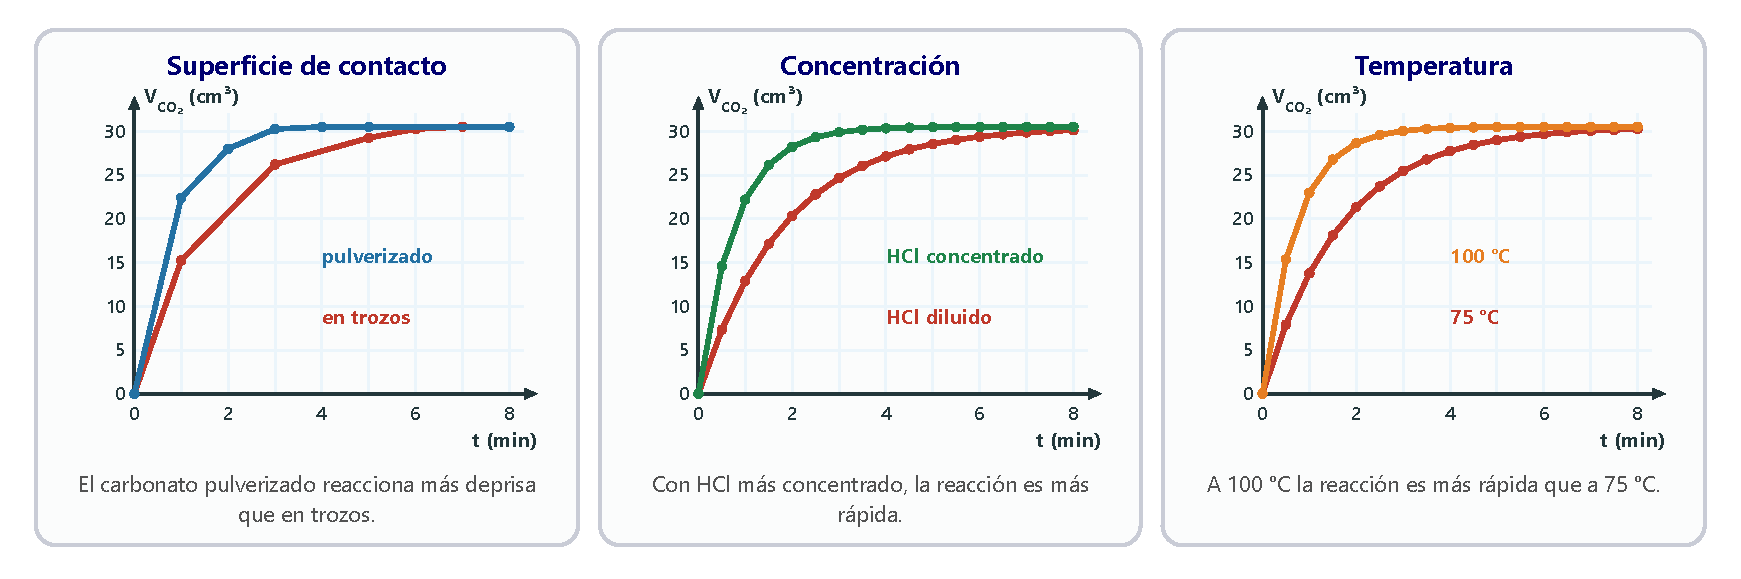
\includegraphics[width=\textwidth]{images/UD6/factores_velocidad}
    \caption{Volumen de \ch{CO2} desprendido frente al tiempo al variar la superficie de contacto, la concentración del ácido y la temperatura.}
    \label{fig:factores_velocidad}
\end{figure}

\paragraph{¿Cómo lo explica la teoría de las colisiones?} La velocidad depende del número de \textbf{choques eficaces} por unidad de tiempo (figura~\ref{fig:particulas_velocidad}):
\begin{itemize}
    \item Si el sólido está más dividido, hay más partículas en la superficie que pueden chocar.
    \item Si la concentración es mayor, hay más partículas en el mismo volumen y chocan más a menudo.
    \item Si la temperatura es mayor, las partículas se mueven más deprisa: chocan más veces y una proporción mayor de los choques tiene la energía suficiente.
    \item Un catalizador positivo permite que la reacción transcurra por un camino con un complejo activado de \textbf{menor energía de activación}; uno negativo, por un camino de mayor energía de activación (figura~\ref{fig:catalizador}).
\end{itemize}

\begin{figure}[H]
    \centering
    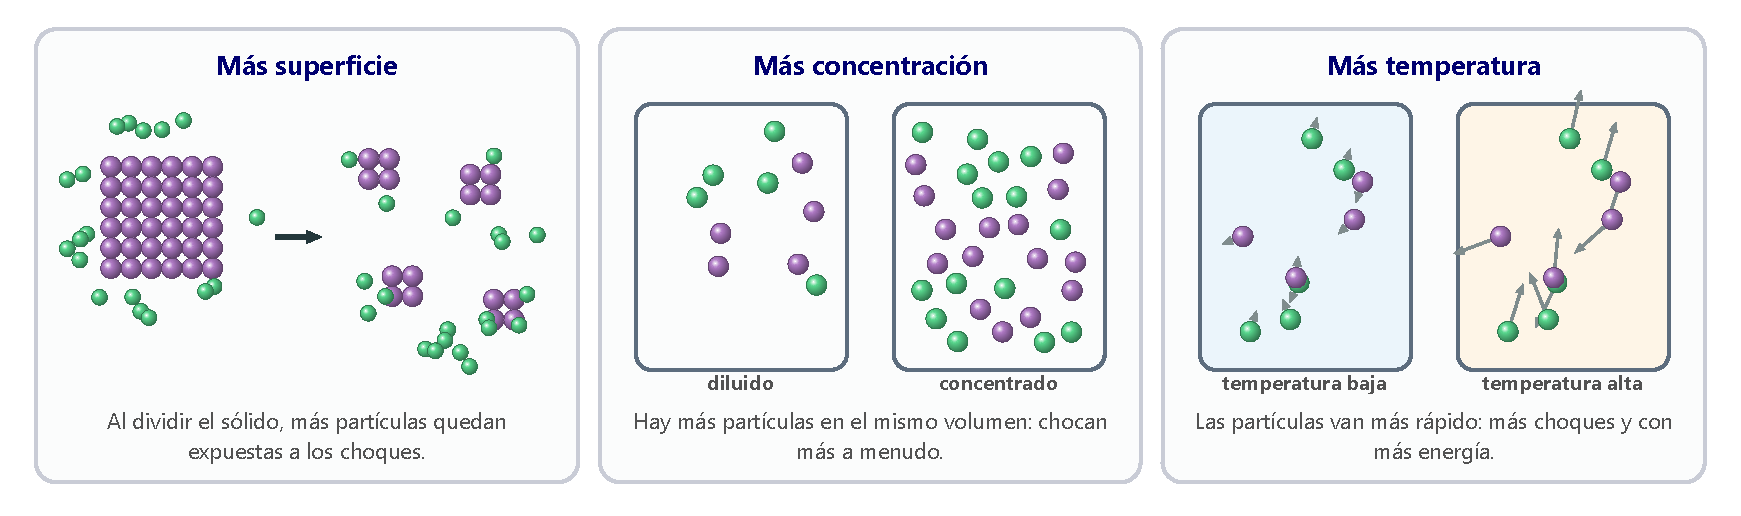
\includegraphics[width=\textwidth]{images/UD6/particulas_velocidad}
    \caption{Interpretación de los factores que afectan a la velocidad con el modelo de partículas.}
    \label{fig:particulas_velocidad}
\end{figure}

\begin{figure}[H]
    \centering
    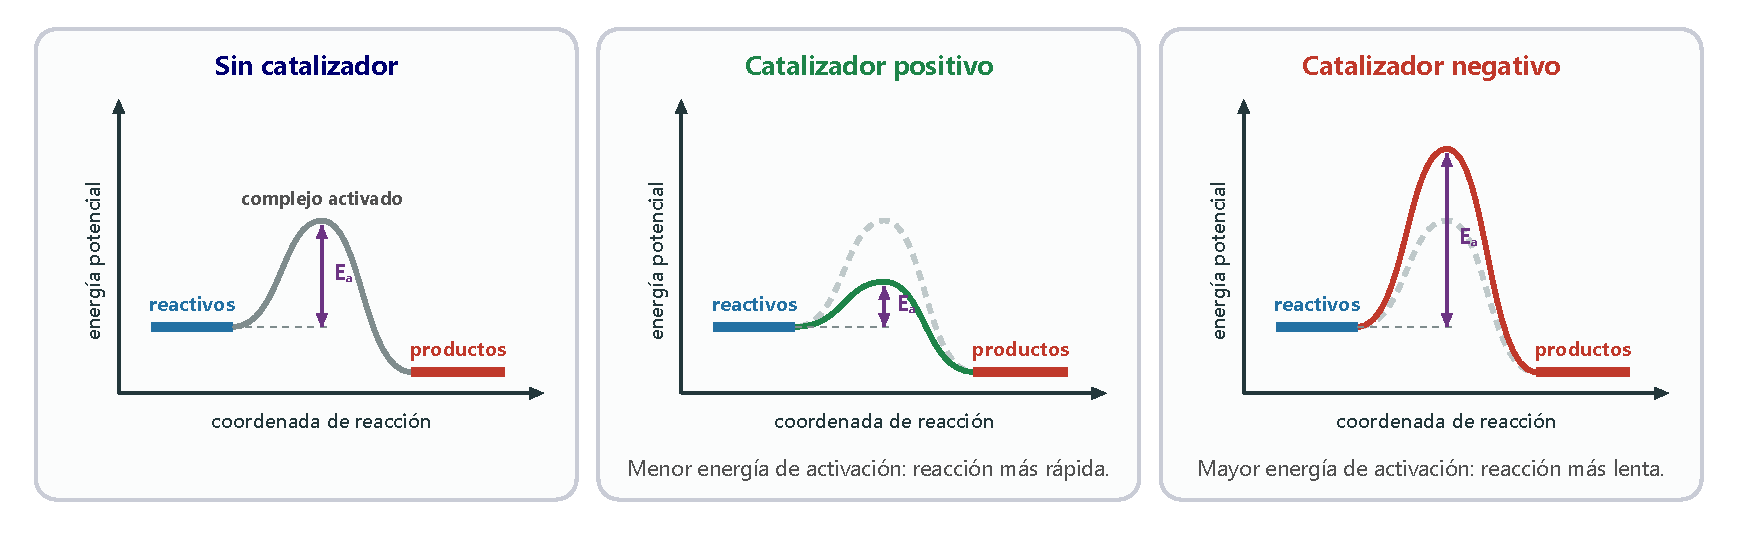
\includegraphics[width=\textwidth]{images/UD6/catalizador}
    \caption{Los catalizadores modifican la energía de activación de una reacción.}
    \label{fig:catalizador}
\end{figure}

\begin{exercise}
    Con los datos de la tabla, ¿qué volumen de \ch{CO2} se ha obtenido a los 3 minutos en cada experimento? ¿Cuál ha sido la velocidad media de la reacción hasta ese momento?
    \begin{solu}
        En trozos: \qty{26.20}{\cubic\centi\metre}; \(v_m = \frac{\num{26.20}}{3} = \textcolor{red}{\qty{8.73}{\cubic\centi\metre\per\minute}}\). Pulverizado: \qty{30.25}{\cubic\centi\metre}; \(v_m = \frac{\num{30.25}}{3} = \textcolor{red}{\qty{10.08}{\cubic\centi\metre\per\minute}}\).
    \end{solu}
\end{exercise}

\begin{exercise}
    Usa la gráfica de la superficie de contacto (figura~\ref{fig:factores_velocidad}) para responder:
    \begin{enumerate}[label=\alph*)]
        \item ¿Qué volumen de \ch{CO2} se ha obtenido a los 5 minutos en cada caso?
        \item ¿Cuánto tiempo hace falta, aproximadamente, para obtener \qty{15}{\cubic\centi\metre} de \ch{CO2} en cada caso?
        \item ¿Cuál es la velocidad media durante los dos primeros minutos con el carbonato pulverizado? ¿Coincide con la velocidad media de toda la reacción?
    \end{enumerate}
    \begin{solu}
        a) En trozos, \textcolor{red}{\qty{29.25}{\cubic\centi\metre}}; pulverizado, \textcolor{red}{\qty{30.50}{\cubic\centi\metre}} (la reacción ya ha terminado).
        b) En trozos, \textcolor{red}{alrededor de \qty{1}{\minute}}; pulverizado, \textcolor{red}{unos \qty{0.7}{\minute}} (40 segundos).
        c) \(v_m = \frac{28}{2} = \textcolor{red}{\qty{14}{\cubic\centi\metre\per\minute}}\). \textcolor{red}{No}: la velocidad media de toda la reacción es menor, porque la reacción se va frenando a medida que se gastan los reactivos.
    \end{solu}
\end{exercise}

\begin{exercise}
    ¿Por qué la carne picada se estropea antes que la misma cantidad de carne en un solo trozo?
    \begin{solu}
        Porque está más dividida: tiene \textcolor{red}{más superficie de contacto} con el aire y los microorganismos, y las reacciones de descomposición son más rápidas.
    \end{solu}
\end{exercise}

\begin{exercise}
    Algunas manchas desaparecen al tratarlas con lejía. ¿Cómo afectará a la velocidad de esta reacción usar lejía más concentrada? ¿Y lavar la prenda con agua caliente?
    \begin{solu}
        En los dos casos la reacción será \textcolor{red}{más rápida}: al aumentar la concentración hay más choques entre partículas, y al aumentar la temperatura los choques son más frecuentes y más energéticos. (También se decolorará antes el tejido.)
    \end{solu}
\end{exercise}

\begin{exercise}
    ¿Cómo influye la temperatura en la conservación de los alimentos frescos?
    \begin{solu}
        Al bajar la temperatura \textcolor{red}{disminuye la velocidad} de las reacciones de descomposición; por eso los alimentos se conservan más tiempo en el frigorífico o en el congelador.
    \end{solu}
\end{exercise}

\begin{exercise}
    Investiga para qué sirve el catalizador del tubo de escape de los coches.
    \begin{solu}
        Respuesta libre. Acelera reacciones que transforman gases tóxicos de la combustión (\ch{CO}, óxidos de nitrógeno, hidrocarburos sin quemar) en gases menos dañinos (\ch{CO2}, \ch{N2}, \ch{H2O}).
    \end{solu}
\end{exercise}

\begin{exercise}
    El agua oxigenada se descompone muy lentamente: \ch{2 H2O2 (aq) -> 2 H2O (l) + O2 (g)}. Recoger \qty{50}{\cubic\centi\metre} de oxígeno lleva cientos de días; pero si se añade \qty{1}{\gram} de dióxido de manganeso, \ch{MnO2}, basta con unos minutos.
    \begin{enumerate}[label=\alph*)]
        \item Explica lo que ocurre.
        \item ¿Se gasta el dióxido de manganeso?
    \end{enumerate}
    \begin{solu}
        a) El \ch{MnO2} actúa como \textcolor{red}{catalizador positivo}: disminuye la energía de activación y la reacción se acelera. b) \textcolor{red}{No}: al final se recupera el gramo de \ch{MnO2} sin cambios.
    \end{solu}
\end{exercise}

\begin{exercise}
    Al mezclar ácido clorhídrico con tiosulfato de sodio se forma un precipitado amarillo de azufre. Colocamos el vaso sobre un papel con una cruz dibujada y medimos el tiempo que tarda en dejar de verse la cruz. Repetimos el experimento con las mismas concentraciones a distintas temperaturas:
    \begin{center}
        % --- tabla antigua ---
        % \begin{tblr}{colspec={lcccc}, hlines, vlines, column{1}={bg=ocre!85, fg=white, font=\bfseries}}
            % Temperatura (\unit{\celsius}) & 15 & 25 & 35 & 45 \\
            % Tiempo (\unit{\second}) & 240 & 130 & 60 & 35 \\
        % \end{tblr}
        % --- tabla nueva ---
        \begin{tabular}{@{}lcccc@{}}
            \toprule
            \textbf{Temperatura (\unit{\celsius})} & 15 & 25 & 35 & 45 \\[3pt]
            \textbf{Tiempo (\unit{\second})} & 240 & 130 & 60 & 35 \\
            \bottomrule
        \end{tabular}
    \end{center}
    \begin{enumerate}[label=\alph*)]
        \item ¿Qué conclusión sacas sobre la velocidad de la reacción?
        \item ¿Por qué hay que mantener constantes las concentraciones?
    \end{enumerate}
    \begin{solu}
        a) Cuanto mayor es la temperatura, menos tarda en desaparecer la cruz: la velocidad \textcolor{red}{aumenta con la temperatura}.
        b) Porque queremos estudiar solo el efecto de la temperatura: es la \textcolor{red}{variable independiente}, y la concentración es una variable controlada. Si cambiaran las dos a la vez, no sabríamos a cuál se debe el efecto.
    \end{solu}
\end{exercise}

\begin{exercise}
    Lee el texto y responde:

    \begin{quote}
        \emph{Una mezcla de hidrógeno y oxígeno puede estar en un recipiente durante años sin cambio aparente: a temperatura ambiente reaccionan, pero con una lentitud extraordinaria. Si se calienta, las paredes se empañan de agua, y a unos \qty{550}{\celsius} la mezcla explota. Hace más de un siglo se comprobó que, si se introduce un alambre de platino en la mezcla fría, la reacción se completa en segundos y el platino sale intacto.}
    \end{quote}

    \begin{enumerate}[label=\alph*)]
        \item ¿Una explosión es una reacción exotérmica o endotérmica?
        \item ¿Cómo es la velocidad de la reacción a temperatura ambiente? ¿Y a \qty{550}{\celsius}?
        \item Escribe la ecuación ajustada de formación del agua.
        \item ¿Qué factores influyen en su velocidad según el texto? ¿Qué papel tiene el platino?
    \end{enumerate}
    \begin{solu}
        a) \textcolor{red}{Exotérmica}: desprende mucha energía y gases muy rápidamente.
        b) A temperatura ambiente es \textcolor{red}{extremadamente lenta}; a \qty{550}{\celsius} es \textcolor{red}{explosiva}.
        c) \ch{2 H2 (g) + O2 (g) -> 2 H2O (g)}.
        d) La \textcolor{red}{temperatura} y la presencia de un \textcolor{red}{catalizador}: el platino acelera la reacción y no se gasta.
    \end{solu}
\end{exercise}

%========================================================================================
\section{Reacciones exotérmicas y endotérmicas}
%========================================================================================

Si añadimos ácido clorhídrico a unas limaduras de zinc, la temperatura sube y el vaso se calienta. En toda reacción química se desprende o se absorbe energía, normalmente en forma de calor, de luz o de electricidad.

\begin{definition}[Reacciones exotérmicas y endotérmicas]
    Una reacción es \textbf{exotérmica} si \textbf{desprende} energía, y \textbf{endotérmica} si la \textbf{absorbe}. El \textbf{calor de reacción} es la energía en forma de calor que se desprende o se absorbe en una reacción.
\end{definition}

En una reacción exotérmica los productos tienen \textbf{menos} energía que los reactivos, y la diferencia se desprende. En una endotérmica los productos tienen \textbf{más} energía, y la diferencia hay que aportarla (figura~\ref{fig:exo_endo}).

\begin{figure}[H]
    \centering
    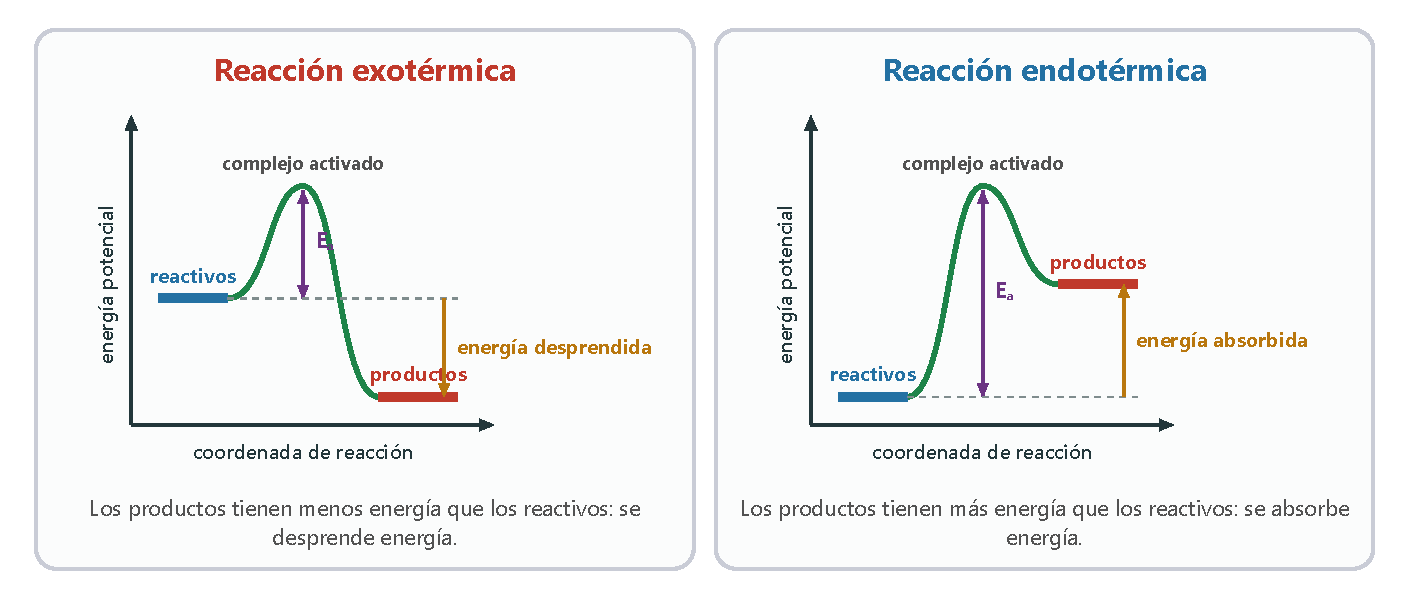
\includegraphics[width=0.9\textwidth]{images/UD6/exo_endo}
    \caption{Diagramas de energía de una reacción exotérmica y de una endotérmica.}
    \label{fig:exo_endo}
\end{figure}

\subsection{Ecuaciones termoquímicas}

Una \textbf{ecuación termoquímica} es una ecuación química ajustada en la que se indica la energía desprendida o absorbida y el estado físico de todas las sustancias. Por convenio, la energía es \textbf{negativa} si la reacción es \textbf{exotérmica} y \textbf{positiva} si es \textbf{endotérmica}:
\begin{align*}
    &\ch{H2 (g) + 1/2 O2 (g) -> H2O (g)} \qquad \text{calor de reacción} = \qty{-241.8}{\kilo\joule\per\mol} \\
    &\ch{CaCO3 (s) -> CaO (s) + CO2 (g)} \qquad \text{calor de reacción} = \qty{+178}{\kilo\joule\per\mol}
\end{align*}
La primera indica que al formarse \qty{1}{\mol} de agua se desprenden \qty{241.8}{\kilo\joule}; la segunda, que para descomponer \qty{1}{\mol} de carbonato de calcio hay que aportar \qty{178}{\kilo\joule}.

\begin{remark}
    \textbf{Reacciones reversibles e irreversibles.} Una reacción es \textbf{reversible} si, a medida que se forman los productos, estos reaccionan entre sí y vuelven a dar los reactivos; se llega a un \emph{equilibrio} dinámico y se escribe con una doble flecha: \(\ch{H2 + I2 <=> 2 HI}\). Es \textbf{irreversible} si los productos no reaccionan entre sí, como cuando se forma un precipitado que se separa: \(\ch{AgNO3 (aq) + NaCl (aq) -> AgCl (s) v + NaNO3 (aq)}\).
\end{remark}

\begin{exercise}
    Clasifica estas reacciones en exotérmicas y endotérmicas:
    \begin{enumerate}[label=\alph*)]
        \item \ch{N2 + 3 H2 -> 2 NH3}; calor de reacción: \qty{-92}{\kilo\joule}
        \item \ch{N2 + O2 -> 2 NO}; calor de reacción: \qty{+181}{\kilo\joule}
        \item \ch{2 SO2 + O2 -> 2 SO3}; calor de reacción: \qty{-198}{\kilo\joule}
        \item \ch{2 H2O -> 2 H2 + O2}; calor de reacción: \qty{+484}{\kilo\joule}
    \end{enumerate}
    \begin{solu}
        Exotérmicas (energía negativa): \textcolor{red}{a) y c)}. Endotérmicas (energía positiva): \textcolor{red}{b) y d)}.
    \end{solu}
\end{exercise}

\begin{exercise}
    Con la ecuación termoquímica de formación del agua, ¿qué energía se desprende al formarse \qty{1.5}{\mol} de agua? ¿Y al reaccionar \qty{4}{\gram} de hidrógeno?
    \begin{solu}
        \(\num{1.5} \cdot \num{241.8} = \textcolor{red}{\qty{362.7}{\kilo\joule}}\). \qty{4}{\gram} de \ch{H2} son \qty{2}{\mol}, que forman \qty{2}{\mol} de agua: \(2 \cdot \num{241.8} = \textcolor{red}{\qty{483.6}{\kilo\joule}}\).
    \end{solu}
\end{exercise}

\begin{exercise}
    Indica si son verdaderas o falsas y corrige las falsas:
    \begin{enumerate}[label=\alph*)]
        \item Una reacción exotérmica absorbe energía.
        \item En una reacción exotérmica la energía se considera positiva.
        \item En una reacción endotérmica la energía se considera negativa.
        \item El calor de reacción es la energía que se absorbe o se desprende en una reacción.
        \item Si el calor de reacción es \qty{-125}{\kilo\joule\per\mol}, se absorben \qty{125}{\kilo\joule} por mol.
        \item En una reacción exotérmica los productos tienen menos energía que los reactivos.
        \item En una reacción endotérmica los productos tienen menos energía que los reactivos.
    \end{enumerate}
    \begin{solu}
        a) \textcolor{red}{Falsa}: la \emph{desprende}. b) \textcolor{red}{Falsa}: se considera \emph{negativa}. c) \textcolor{red}{Falsa}: se considera \emph{positiva}. d) \textcolor{red}{Verdadera}. e) \textcolor{red}{Falsa}: se \emph{desprenden} \qty{125}{\kilo\joule} por mol. f) \textcolor{red}{Verdadera}. g) \textcolor{red}{Falsa}: tienen \emph{más} energía.
    \end{solu}
\end{exercise}

\begin{exercise}
    Dibuja el diagrama de energía de una reacción exotérmica y el de una endotérmica. Indica en ellos: a) las magnitudes de los ejes; b) dónde están los reactivos y los productos; c) la energía de activación; d) la energía desprendida o absorbida.
    \begin{solu}
        Como los de la figura~\ref{fig:exo_endo}: a) eje vertical, \textcolor{red}{energía}; eje horizontal, \textcolor{red}{coordenada (avance) de la reacción}. b) Reactivos a la izquierda y productos a la derecha; en la exotérmica los productos quedan más abajo y en la endotérmica, más arriba. c) La energía de activación es la altura desde los reactivos hasta la cima (complejo activado). d) La energía desprendida o absorbida es la diferencia de altura entre reactivos y productos.
    \end{solu}
\end{exercise}

\begin{exercise}
    Para la reacción \ch{H2 (g) + Cl2 (g) -> 2 HCl (g)} se desprenden \qty{184}{\kilo\joule}.
    \begin{enumerate}[label=\alph*)]
        \item ¿Es exotérmica o endotérmica?
        \item ¿Qué energía se desprende al formarse \qty{1}{\mol} de \ch{HCl}? ¿Y \qty{3}{\mol}?
        \item Dibuja su diagrama de energía.
    \end{enumerate}
    \begin{solu}
        a) \textcolor{red}{Exotérmica}. b) Por mol de \ch{HCl}: \(\frac{184}{2} = \textcolor{red}{\qty{92}{\kilo\joule}}\); para \qty{3}{\mol}: \(3 \cdot 92 = \textcolor{red}{\qty{276}{\kilo\joule}}\). c) Como el diagrama exotérmico de la figura~\ref{fig:exo_endo}, con \ch{H2 + Cl2} a la izquierda, \ch{2 HCl} \qty{184}{\kilo\joule} más abajo a la derecha.
    \end{solu}
\end{exercise}

\begin{exercise}
    La combustión del carbono es \ch{C (s) + O2 (g) -> CO2 (g)}, con un calor de reacción de \qty{-393.5}{\kilo\joule\per\mol}.
    \begin{enumerate}[label=\alph*)]
        \item ¿Es exotérmica o endotérmica?
        \item ¿Qué energía se desprende al quemar \qty{500}{\gram} de carbono?
    \end{enumerate}
    \begin{solu}
        a) \textcolor{red}{Exotérmica}. b) \(n = \frac{500}{12} = \qty{41.67}{\mol}\); \(E = \num{41.67} \cdot \num{393.5} = \textcolor{red}{\qty{16397}{\kilo\joule}}\) (unos \qty{1.64e4}{\kilo\joule}).
    \end{solu}
\end{exercise}

\begin{exercise}
    En la combustión del metano se desprenden \qty{890}{\kilo\joule\per\mol}, y en la del butano, \qty{2876}{\kilo\joule\per\mol}. Si quemamos \qty{500}{\gram} de cada combustible, ¿cuál desprende más energía?
    \begin{solu}
        Metano (\(M = \qty{16}{\gram\per\mol}\)): \(\frac{500}{16} = \qty{31.25}{\mol}\); \(\num{31.25} \cdot 890 = \qty{27813}{\kilo\joule}\).
        Butano (\(M = \qty{58}{\gram\per\mol}\)): \(\frac{500}{58} = \qty{8.62}{\mol}\); \(\num{8.62} \cdot 2876 = \qty{24793}{\kilo\joule}\).
        Desprende más energía el \textcolor{red}{metano}, aunque por mol desprenda menos.
    \end{solu}
\end{exercise}

\begin{exercise}
    En el diagrama de energía de la reacción \ch{2 NOCl -> 2 NO + Cl2} los productos están por encima de los reactivos. En el de la reacción \ch{NO + O3 -> NO2 + O2} los productos están por debajo. ¿Cuál es exotérmica y cuál endotérmica?
    \begin{solu}
        La primera es \textcolor{red}{endotérmica} (los productos tienen más energía) y la segunda, \textcolor{red}{exotérmica} (los productos tienen menos energía).
    \end{solu}
\end{exercise}

%========================================================================================
\section{Tipos de reacciones químicas}
%========================================================================================

A diario se producen centenares de reacciones: en los laboratorios y en la industria, pero también en la atmósfera, en la cocina o en nuestro cuerpo. Muchas de ellas pueden clasificarse en unos pocos tipos.

\subsection{Reacciones de síntesis}

En una reacción de \textbf{síntesis} dos o más sustancias reaccionan para dar una única sustancia nueva.

\begin{center}
    % --- tabla antigua ---
    % \begin{tblr}{colspec={X[c]X[c]}, hlines, vlines, row{1}={bg=ocre!85, fg=white, font=\bfseries}, rowsep=2pt}
        % A partir de sus elementos & A partir de otros compuestos \\
        % {No metal + metal \(\to\) sal binaria \\ \ch{Cl2 (g) + 2 Na (s)} \(\rightarrow\) \ch{2 NaCl (s)}} & {Óxido de metal + agua \(\to\) hidróxido \\ \ch{CaO (s) + H2O (l)} \(\rightarrow\) \ch{Ca(OH)2 (aq)}} \\
        % {Metal + oxígeno \(\to\) óxido de metal \\ \ch{2 Mg (s) + O2 (g)} \(\rightarrow\) \ch{2 MgO (s)}} & {Óxido de no metal + agua \(\to\) oxoácido \\ \ch{SO3 (g) + H2O (l)} \(\rightarrow\) \ch{H2SO4 (aq)}} \\
        % {No metal + oxígeno \(\to\) óxido de no metal \\ \ch{2 H2 (g) + O2 (g)} \(\rightarrow\) \ch{2 H2O (l)}} & {Compuesto + elemento \(\to\) nuevo compuesto \\ \ch{PCl3 (g) + Cl2 (g)} \(\rightarrow\) \ch{PCl5 (g)}} \\
        % {No metal + no metal \(\to\) hidruro no metálico \\ \ch{N2 (g) + 3 H2 (g)} \(\rightarrow\) \ch{2 NH3 (g)}} & \\
    % \end{tblr}
    % --- tabla nueva ---
    \begin{tabular}{@{}C{0.45\linewidth} C{0.45\linewidth}@{}}
        \toprule
        \textbf{A partir de sus elementos} & \textbf{A partir de otros compuestos} \\
        \midrule
        No metal + metal \(\to\) sal binaria \newline \ch{Cl2 (g) + 2 Na (s)} \(\rightarrow\) \ch{2 NaCl (s)} & Óxido de metal + agua \(\to\) hidróxido \newline \ch{CaO (s) + H2O (l)} \(\rightarrow\) \ch{Ca(OH)2 (aq)} \\[3pt]
        Metal + oxígeno \(\to\) óxido de metal \newline \ch{2 Mg (s) + O2 (g)} \(\rightarrow\) \ch{2 MgO (s)} & Óxido de no metal + agua \(\to\) oxoácido \newline \ch{SO3 (g) + H2O (l)} \(\rightarrow\) \ch{H2SO4 (aq)} \\[3pt]
        No metal + oxígeno \(\to\) óxido de no metal \newline \ch{2 H2 (g) + O2 (g)} \(\rightarrow\) \ch{2 H2O (l)} & Compuesto + elemento \(\to\) nuevo compuesto \newline \ch{PCl3 (g) + Cl2 (g)} \(\rightarrow\) \ch{PCl5 (g)} \\[3pt]
        No metal + no metal \(\to\) hidruro no metálico \newline \ch{N2 (g) + 3 H2 (g)} \(\rightarrow\) \ch{2 NH3 (g)} &  \\
        \bottomrule
    \end{tabular}
\end{center}

\subsection{Reacciones de oxidación y de reducción}

Los objetos de hierro que están a la intemperie se cubren de herrumbre si no se protegen con pintura. Es una \textbf{oxidación}.
\begin{itemize}
    \item Una \textbf{oxidación} es una reacción en la que una sustancia \textbf{gana oxígeno}:
    \[ \ch{2 Fe (s) + O2 (g) -> 2 FeO (s)} \qquad \ch{2 Cu (s) + O2 (g) -> 2 CuO (s)} \]
    \item Una \textbf{reducción} es una reacción en la que un compuesto \textbf{pierde oxígeno}.
\end{itemize}
La oxidación y la reducción ocurren siempre a la vez. En la reacción
\[ \ch{CuO (s) + H2 (g) -> Cu (s) + H2O (g)} \]
el óxido de cobre(II) \textbf{se reduce} (pierde oxígeno) y el hidrógeno \textbf{se oxida} (lo gana). El hidrógeno es el \textbf{agente reductor} y el óxido de cobre, el \textbf{agente oxidante}. En realidad, estas reacciones son \textbf{transferencias de electrones}: la sustancia que cede electrones se oxida y la que los capta se reduce. Por eso se llaman reacciones \textbf{redox}.

\begin{remark}
    \textbf{El enranciamiento y la corrosión.} La mantequilla, el aceite o el vino se \emph{enrancian} al oxidarse; por eso se guardan en lugares frescos y oscuros, y muchos alimentos llevan antioxidantes. La \emph{corrosión} es la oxidación del hierro y del acero no protegidos: destruye estructuras metálicas y prevenirla tiene un coste elevado.
\end{remark}

\subsection{Los procesos electroquímicos}

Los procesos \textbf{electroquímicos} transforman energía química en eléctrica, o al revés (figura~\ref{fig:pila_electrolisis}).
\begin{itemize}
    \item \textbf{Las pilas.} En una reacción redox hay una transferencia de electrones. Si la oxidación y la reducción tienen lugar en sitios separados y unidos por un circuito, los electrones circulan por él: se produce una corriente eléctrica continua. Es una \textbf{pila}. En la \emph{pila alcalina}, el zinc del electrodo negativo se oxida a \ch{Zn^{2+}} y el dióxido de manganeso, en contacto con la barra de grafito del electrodo positivo, capta los electrones y se reduce.
    \item \textbf{La electrólisis.} Si hacemos pasar corriente eléctrica a través de un compuesto iónico fundido o disuelto (el \textbf{electrolito}), se produce una reacción química, inversa a la de una pila. Hacen falta un generador de corriente continua, el electrolito, una cuba electrolítica y dos electrodos (cátodo y ánodo). La electrólisis del agua produce hidrógeno y oxígeno: \(\ch{2 H2O (l) -> 2 H2 (g) + O2 (g)}\).
\end{itemize}

\begin{figure}[H]
    \centering
    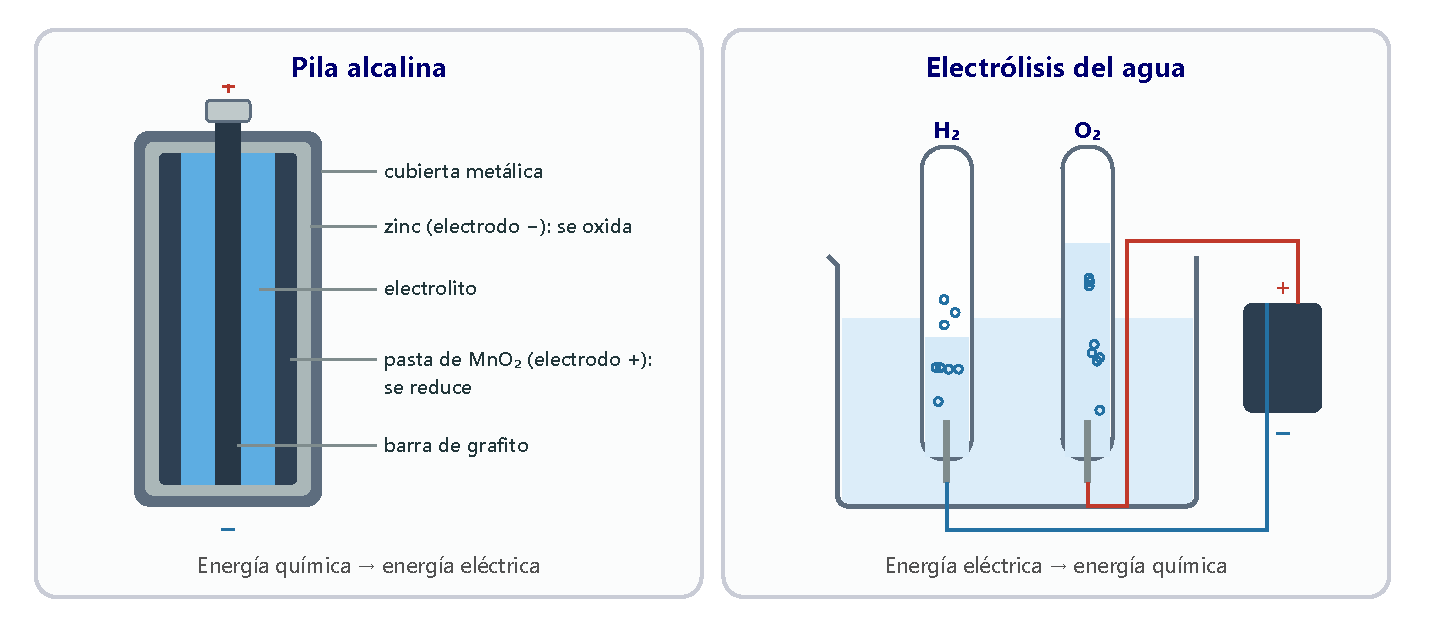
\includegraphics[width=0.95\textwidth]{images/UD6/pila_electrolisis}
    \caption{Una pila transforma energía química en eléctrica; la electrólisis hace lo contrario.}
    \label{fig:pila_electrolisis}
\end{figure}

\paragraph{Aplicaciones de la electrólisis.} Permite obtener elementos a partir de sus compuestos: cobre muy puro, hidrógeno para usarlo como combustible («hidrógeno verde» si la electricidad es renovable), o metales como el aluminio, el sodio o el magnesio. También se usa en la \textbf{galvanoplastia}: recubrir un objeto metálico con otro metal (plata, oro, níquel) para decorarlo o protegerlo, colocándolo como cátodo en una disolución con iones de ese metal.

\subsection{Ácidos y bases}

El químico sueco Svante \textbf{Arrhenius} (1859-1927) dio la primera definición de ácido y de base basándose en su disociación en agua:

\begin{center}
    % --- tabla antigua ---
    % \begin{tblr}{colspec={X[l]X[l]}, hlines, vlines, row{1}={bg=ocre!85, fg=white, font=\bfseries, halign=c}}
        % Ácido & Base \\
        % {Sustancia que en disolución acuosa se disocia dando \textbf{iones hidrógeno}, \ch{H+}: \\ \ch{HCl (aq)} \(\rightarrow\) \ch{H+ (aq) + Cl- (aq)}} & {Sustancia que en disolución acuosa se disocia dando \textbf{iones hidróxido}, \ch{OH-}: \\ \ch{NaOH (aq)} \(\rightarrow\) \ch{Na+ (aq) + OH- (aq)}} \\
        % Sabor ácido. Reaccionan con metales como el zinc o el magnesio desprendiendo hidrógeno. Reaccionan con las bases para dar sales. & Sabor amargo. Reaccionan con los ácidos para dar sales. Reaccionan con las grasas formando jabones. \\
        % Ejemplos: ácido clorhídrico, nítrico, sulfúrico, acético (vinagre)\ldots & Ejemplos: amoníaco, hidróxidos de los metales alcalinos y alcalinotérreos\ldots \\
    % \end{tblr}
    % --- tabla nueva ---
    \begin{tabular}{@{}L{0.45\linewidth} L{0.45\linewidth}@{}}
        \toprule
        \textbf{Ácido} & \textbf{Base} \\
        \midrule
        Sustancia que en disolución acuosa se disocia dando \textbf{iones hidrógeno}, \ch{H+}: \newline \ch{HCl (aq)} \(\rightarrow\) \ch{H+ (aq) + Cl- (aq)} & Sustancia que en disolución acuosa se disocia dando \textbf{iones hidróxido}, \ch{OH-}: \newline \ch{NaOH (aq)} \(\rightarrow\) \ch{Na+ (aq) + OH- (aq)} \\[3pt]
        Sabor ácido. Reaccionan con metales como el zinc o el magnesio desprendiendo hidrógeno. Reaccionan con las bases para dar sales. & Sabor amargo. Reaccionan con los ácidos para dar sales. Reaccionan con las grasas formando jabones. \\[3pt]
        Ejemplos: ácido clorhídrico, nítrico, sulfúrico, acético (vinagre)\ldots & Ejemplos: amoníaco, hidróxidos de los metales alcalinos y alcalinotérreos\ldots \\
        \bottomrule
    \end{tabular}
\end{center}

\paragraph{La escala de pH.} Es una escala numérica, normalmente entre 0 y 14, que indica el grado de acidez o basicidad de una disolución (figura~\ref{fig:escala_ph}):
\begin{itemize}
    \item pH = 7: disolución \textbf{neutra}.
    \item pH < 7: disolución \textbf{ácida} (cuanto menor, más ácida).
    \item pH > 7: disolución \textbf{básica} (cuanto mayor, más básica).
\end{itemize}
El pH se mide con \textbf{indicadores} (como la fenolftaleína, incolora en medio ácido y rosa en medio básico), con \textbf{papel indicador}, que cambia de color, o con un \textbf{pH-metro} digital.

\begin{figure}[H]
    \centering
    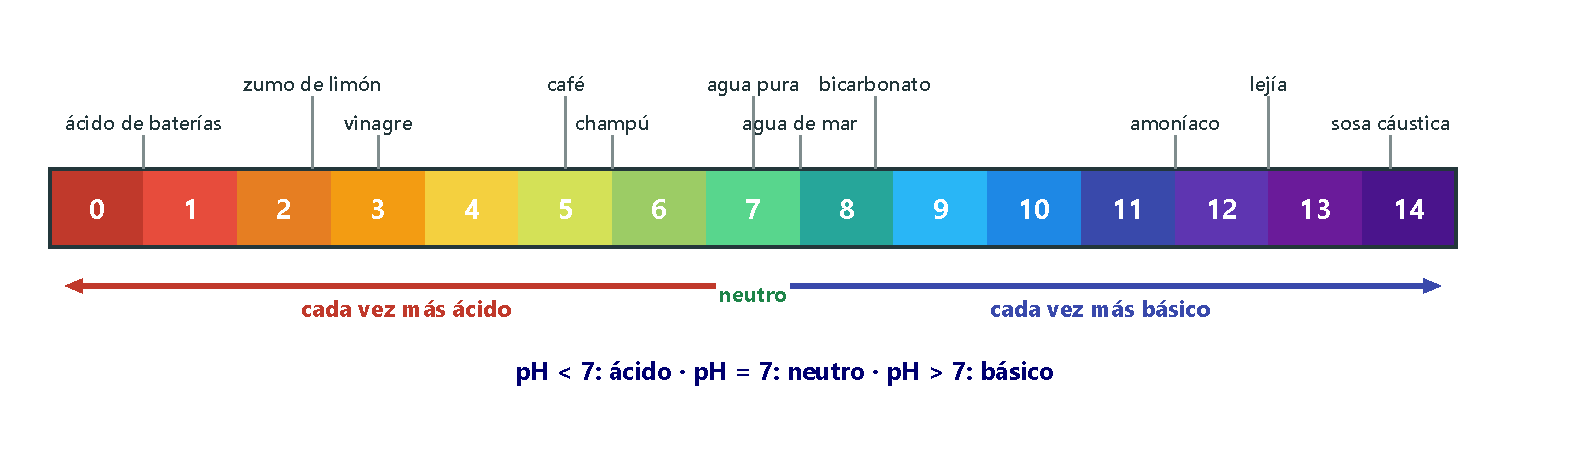
\includegraphics[width=\textwidth]{images/UD6/escala_ph}
    \caption{Escala de pH con algunas sustancias de uso cotidiano.}
    \label{fig:escala_ph}
\end{figure}

\paragraph{La neutralización.} Es la reacción entre un ácido y una base para dar una \textbf{sal y agua}. Si añadimos poco a poco ácido clorhídrico a una disolución de hidróxido de sodio, llega un momento en que la disolución es neutra:
\[ \text{ácido} + \text{base} \longrightarrow \text{sal} + \text{agua} \qquad \ch{HCl (aq) + NaOH (aq) -> NaCl (aq) + H2O (l)} \]

\subsection{Reacciones de combustión}

Una \textbf{combustión} es una oxidación muy rápida en la que una sustancia (el combustible) reacciona con el oxígeno y se desprende mucha energía: es una reacción \textbf{exotérmica}. Por eso se usa para obtener energía en los hogares, los motores, la industria y las centrales térmicas. Los combustibles más usados son el metano (gas natural), el propano, el butano, la gasolina, el gasóleo y otros derivados del petróleo.
\begin{itemize}
    \item Combustión del carbono: \(\ch{C (s) + O2 (g) -> CO2 (g)} + \text{energía}\)
    \item Combustión de un hidrocarburo: \(\ch{CH4 (g) + 2 O2 (g) -> CO2 (g) + 2 H2O (l)} + \text{energía}\)
    \item Respiración celular: \(\ch{C6H12O6 (aq) + 6 O2 (g) -> 6 CO2 (g) + 6 H2O (l)} + \text{energía}\)
\end{itemize}

\paragraph{El efecto invernadero.} Algunos gases de la atmósfera, como el \ch{CO2}, el metano o el vapor de agua, retienen parte del calor que emite la superficie terrestre y lo devuelven hacia ella. Este \textbf{efecto invernadero} natural mantiene una temperatura adecuada para la vida. Pero desde la Revolución Industrial, la quema de combustibles fósiles ha aumentado mucho el \ch{CO2} atmosférico: es el \textbf{incremento del efecto invernadero}, que provoca un aumento de la temperatura media de la Tierra (\textbf{calentamiento global}). Una de sus consecuencias es el \textbf{cambio climático}: un cambio global en las pautas del clima.

\begin{figure}[H]
    \centering
    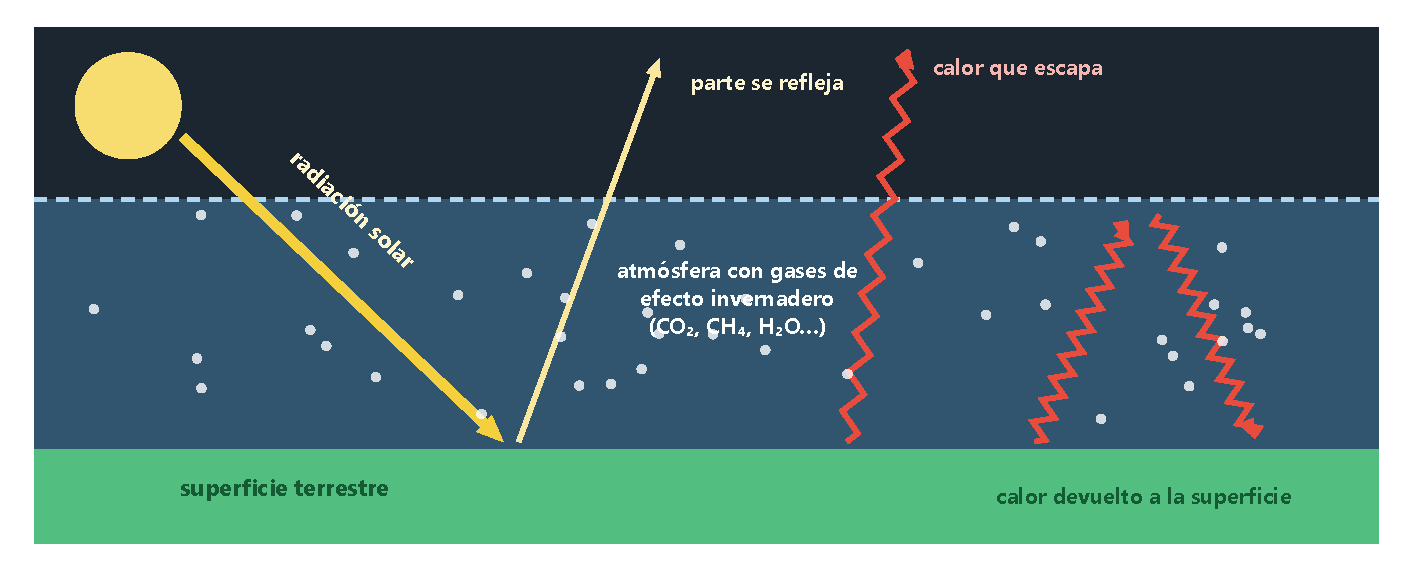
\includegraphics[width=0.9\textwidth]{images/UD6/efecto_invernadero}
    \caption{El efecto invernadero: parte del calor emitido por la Tierra vuelve hacia la superficie.}
    \label{fig:efecto_invernadero}
\end{figure}

\begin{exercise}
    Escribe la ecuación de disociación en agua de estas sustancias e indica cuáles son ácidos y cuáles bases: a) ácido bromhídrico, \ch{HBr}; b) ácido acético, \ch{CH3COOH}; c) hidróxido de sodio, \ch{NaOH}; d) hidróxido de bario, \ch{Ba(OH)2}.
    \begin{solu}
        a) \ch{HBr (aq) -> H+ (aq) + Br- (aq)}: \textcolor{red}{ácido}. b) \ch{CH3COOH (aq) -> H+ (aq) + CH3COO- (aq)}: \textcolor{red}{ácido}. c) \ch{NaOH (aq) -> Na+ (aq) + OH- (aq)}: \textcolor{red}{base}. d) \ch{Ba(OH)2 (aq) -> Ba^{2+} (aq) + 2 OH- (aq)}: \textcolor{red}{base}.
    \end{solu}
\end{exercise}

\begin{exercise}
    Clasifica en ácidas, neutras o básicas estas sustancias según su pH: leche, \num{6.5}; lejía, \num{12.5}; refresco de cola, \num{2.5}; sangre, \num{7.4}; vinagre, 3; agua destilada, 7.
    \begin{solu}
        Ácidas: \textcolor{red}{leche, refresco de cola y vinagre}. Neutra: \textcolor{red}{agua destilada}. Básicas: \textcolor{red}{lejía y sangre}.
    \end{solu}
\end{exercise}

\begin{exercise}
    Escribe una reacción de neutralización con la que se pueda obtener: a) cloruro de potasio; b) bromuro de calcio; c) nitrato de potasio; d) sulfato de sodio.
    \begin{solu}
        a) \ch{HCl (aq) + KOH (aq) -> KCl (aq) + H2O (l)}
        \quad b) \ch{2 HBr (aq) + Ca(OH)2 (aq) -> CaBr2 (aq) + 2 H2O (l)}

        c) \ch{HNO3 (aq) + KOH (aq) -> KNO3 (aq) + H2O (l)}
        \quad d) \ch{H2SO4 (aq) + 2 NaOH (aq) -> Na2SO4 (aq) + 2 H2O (l)}
    \end{solu}
\end{exercise}

\begin{exercise}
    Completa estas reacciones de neutralización:
    \begin{enumerate}[label=\alph*)]
        \item \ch{CH3COOH + KOH ->}
        \item \ch{HBr + NaOH ->}
        \item \ch{HCOOH + NaOH ->}
        \item \ch{HNO3 + KOH ->}
    \end{enumerate}
    \begin{solu}
        a) \ch{CH3COOH + KOH -> CH3COOK + H2O}
        \quad b) \ch{HBr + NaOH -> NaBr + H2O}

        c) \ch{HCOOH + NaOH -> HCOONa + H2O}
        \quad d) \ch{HNO3 + KOH -> KNO3 + H2O}
    \end{solu}
\end{exercise}

\begin{exercise}
    Clasifica estas reacciones como de síntesis, de neutralización o de combustión (alguna puede ser de dos tipos):
    \begin{enumerate}[label=\alph*)]
        \item \ch{CaO (s) + H2O (l) -> Ca(OH)2 (aq)}
        \item \ch{C3H8 (g) + 5 O2 (g) -> 3 CO2 (g) + 4 H2O (l)}
        \item \ch{HNO3 (aq) + KOH (aq) -> KNO3 (aq) + H2O (l)}
        \item \ch{C (s) + O2 (g) -> CO2 (g)}
        \item \ch{SO3 (g) + H2O (l) -> H2SO4 (aq)}
        \item \ch{H2SO4 (aq) + Ca(OH)2 (aq) -> CaSO4 (aq) + 2 H2O (l)}
    \end{enumerate}
    \begin{solu}
        Síntesis: \textcolor{red}{a), d) y e)}. Neutralización: \textcolor{red}{c) y f)}. Combustión: \textcolor{red}{b) y d)} (la d es a la vez síntesis y combustión).
    \end{solu}
\end{exercise}

\begin{exercise}
    ¿De qué tipo es cada una de estas reacciones?
    \begin{enumerate}[label=\alph*)]
        \item Un metal y un no metal forman una sal binaria.
        \item Un metal reacciona con oxígeno para dar un óxido.
        \item Un hidrocarburo reacciona con oxígeno para dar dióxido de carbono y agua.
        \item Un óxido de metal reacciona con agua para dar un hidróxido.
    \end{enumerate}
    \begin{solu}
        a) \textcolor{red}{Síntesis}. b) \textcolor{red}{Oxidación} (y también síntesis). c) \textcolor{red}{Combustión}. d) \textcolor{red}{Síntesis}.
    \end{solu}
\end{exercise}

\begin{exercise}
    Indica si son verdaderas o falsas y justifícalo:
    \begin{enumerate}[label=\alph*)]
        \item Una base es una sustancia que en agua se disocia dando iones hidrógeno.
        \item Una sustancia de pH \num{8.2} es básica.
        \item Un champú es neutro si su pH es 7.
        \item La fenolftaleína es rosa en medio ácido.
        \item Una neutralización es una reacción entre dos sustancias neutras.
    \end{enumerate}
    \begin{solu}
        a) \textcolor{red}{Falsa}: da iones \emph{hidróxido}, \ch{OH-}. b) \textcolor{red}{Verdadera}: su pH es mayor que 7. c) \textcolor{red}{Verdadera}. d) \textcolor{red}{Falsa}: es rosa en medio \emph{básico} e incolora en medio ácido. e) \textcolor{red}{Falsa}: es la reacción entre un \emph{ácido} y una \emph{base}, que da sal y agua.
    \end{solu}
\end{exercise}

\begin{exercise}
    En la reacción \ch{ZnO (s) + C (s) -> Zn (s) + CO (g)}, ¿qué sustancia se oxida y cuál se reduce? ¿Cuál es el agente reductor?
    \begin{solu}
        El \ch{ZnO} pierde oxígeno: \textcolor{red}{se reduce}. El carbono gana oxígeno: \textcolor{red}{se oxida}, y es el \textcolor{red}{agente reductor}.
    \end{solu}
\end{exercise}

\begin{exercise}
    Busca información sobre las aplicaciones de la electrólisis. ¿Cómo debemos desechar las pilas gastadas? ¿Por qué?
    \begin{solu}
        Respuesta libre. Las pilas deben depositarse en los \textcolor{red}{contenedores específicos} (puntos limpios, comercios), porque contienen metales pesados y otras sustancias contaminantes que no deben llegar al suelo ni al agua, y que además pueden reciclarse.
    \end{solu}
\end{exercise}

\begin{exercise}
    Distingue entre efecto invernadero e incremento del efecto invernadero. ¿Qué relación tiene este último con el calentamiento global y con el cambio climático?
    \begin{solu}
        El \textcolor{red}{efecto invernadero} es natural: algunos gases atmosféricos retienen parte del calor emitido por la Tierra y mantienen una temperatura adecuada para la vida. Su \textcolor{red}{incremento} se debe al aumento de gases como el \ch{CO2} por la quema de combustibles fósiles, y provoca una subida de la temperatura media del planeta: el \textcolor{red}{calentamiento global}, cuya consecuencia es el \textcolor{red}{cambio climático}.
    \end{solu}
\end{exercise}

\begin{exercise}
    Busca información sobre las aplicaciones de las reacciones de combustión y sus consecuencias, tanto locales (contaminación de las ciudades) como globales.
    \begin{solu}
        Respuesta libre. Aplicaciones: calefacción, cocina, transporte, industria, centrales térmicas. Consecuencias locales: contaminación del aire (\ch{CO}, óxidos de nitrógeno y de azufre, partículas), lluvia ácida. Globales: incremento del efecto invernadero y calentamiento global.
    \end{solu}
\end{exercise}

%========================================================================================
\section{La industria química}
%========================================================================================

La \textbf{industria química} transforma los recursos naturales en sustancias con características diferentes. Las reacciones son las mismas que en el laboratorio, pero los aparatos se diseñan para trabajar con grandes cantidades. Todo proceso químico industrial tiene tres etapas:
\begin{enumerate}[label=\numberballblue]
    \item Preparación de las sustancias que van a reaccionar.
    \item Reacción química propiamente dicha.
    \item Separación y purificación de los productos obtenidos.
\end{enumerate}

\subsection{La industria metalúrgica}

La \textbf{metalurgia} reúne las operaciones necesarias para obtener metales a partir de sus minerales; la del hierro se llama \textbf{siderurgia}. Las etapas son:
\begin{enumerate}[label=\arabic*.]
    \item Extracción del mineral del yacimiento.
    \item Concentración del mineral: se separa la \emph{mena} (la parte útil) de la \emph{ganga} (lo que no interesa) por cribado, trituración, pulverización, lavado\ldots
    \item Conversión de la mena en un óxido, por tostación o calcinación.
    \item Reducción del óxido para liberar el metal. El reductor más usado es el carbón (coque), que se oxida a monóxido o dióxido de carbono:
    \[ \ch{Fe2O3 (s) + 3 C (s) -> 2 Fe (s) + 3 CO (g)} \]
    Los compuestos muy estables (como el cloruro de sodio o el óxido de aluminio) se descomponen por \textbf{electrólisis}, que es muy eficaz pero cara, porque consume mucha electricidad.
    \item Purificación del metal o preparación de una aleación con la composición deseada.
\end{enumerate}

\begin{exercise}
    ¿Cuáles son las etapas de un proceso químico industrial?
    \begin{solu}
        \textcolor{red}{1.} Preparación de los reactivos. \textcolor{red}{2.} Reacción química. \textcolor{red}{3.} Separación y purificación de los productos.
    \end{solu}
\end{exercise}

\begin{exercise}
    Describe los pasos para obtener un metal a partir de su mena. ¿Qué papel tiene el carbón en la siderurgia?
    \begin{solu}
        Extracción del mineral, concentración (separar mena y ganga), conversión de la mena en óxido, reducción del óxido a metal y purificación. El carbón es el \textcolor{red}{agente reductor}: quita el oxígeno al óxido de hierro y se oxida a \ch{CO} o \ch{CO2}.
    \end{solu}
\end{exercise}

\begin{exercise}
    Busca información y elabora un informe sobre las industrias químicas de tu comunidad autónoma. Sitúalas en un mapa.
    \begin{solu}
        Respuesta libre.
    \end{solu}
\end{exercise}
